% Created 2015-01-27 mar 10:21
\documentclass[xcolor={usenames,svgnames,dvipsnames}]{beamer}
\usepackage[utf8]{inputenc}
\usepackage[T1]{fontenc}
\usepackage{fixltx2e}
\usepackage{graphicx}
\usepackage{longtable}
\usepackage{float}
\usepackage{wrapfig}
\usepackage{rotating}
\usepackage[normalem]{ulem}
\usepackage{amsmath}
\usepackage{textcomp}
\usepackage{marvosym}
\usepackage{wasysym}
\usepackage{amssymb}
\usepackage{hyperref}
\tolerance=1000
\usepackage{color}
\usepackage{listings}
\AtBeginSubsection[]{\begin{frame}[plain]\tableofcontents[currentsubsection,sectionstyle=show/shaded,subsectionstyle=show/shaded/hide]\end{frame}}
\lstset{keywordstyle=\color{blue}, commentstyle=\color{gray!90}, basicstyle=\ttfamily\small, columns=fullflexible, breaklines=true,linewidth=\textwidth, backgroundcolor=\color{gray!23}, basewidth={0.5em,0.4em}, literate={á}{{\'a}}1 {ñ}{{\~n}}1 {é}{{\'e}}1 {ó}{{\'o}}1 {º}{{\textordmasculine}}1}
\usepackage{mathpazo}
\hypersetup{colorlinks=true, linkcolor=Blue, urlcolor=Blue}
\usepackage{fancyvrb}
\DefineVerbatimEnvironment{verbatim}{Verbatim}{fontsize=\tiny, formatcom = {\color{black!70}}}
\usetheme{Goettingen}
\usecolortheme{rose}
\usefonttheme{serif}
\author{Oscar Perpiñán Lamigueiro \\ \url{http://oscarperpinan.github.io}}
\date{}
\title{Introducción a R}
\hypersetup{
  pdfkeywords={},
  pdfsubject={},
  pdfcreator={Emacs 24.4.1 (Org mode 8.2.7c)}}
\begin{document}

\maketitle


\section{R es software libre}
\label{sec-1}
\subsection{¿Qué es \texttt{R}?}
\label{sec-1-1}
\begin{frame}[fragile,label=sec-1-1-1]{¿Qué es \texttt{R}?}
 \begin{block}{¿Qué es \href{http://procomun.wordpress.com/2011/02/23/que-es-r/}{R}?}
Es un lenguaje de programación principalmente orientado al
análisis estadístico y visualización de información cuantitativa y
cualitativa y publicado como software libre con licencia GNU-GPL.
\begin{center}
\url{http://www.R-project.org} 
\end{center}
\end{block}
\end{frame}

\begin{frame}[fragile,label=sec-1-1-2]{Para instalar \texttt{R}}
 \begin{itemize}
\item Windows: \url{http://cran.es.r-project.org/bin/windows/base/}
\item Mac: \url{http://cran.es.r-project.org/bin/macosx/}
\item Linux: \url{http://cran.es.r-project.org/bin/linux/}
\end{itemize}
\end{frame}

\begin{frame}[label=sec-1-1-3]{Interfaces para R}
\begin{itemize}
\item En mi opinión, la mejor interfaz para R es \href{http://ess.r-project.org/}{ESS} con \href{http://www.gnu.org/software/emacs/}{Emacs}.
\item Para los que prefieren una interfaz gráfica es recomendable \href{http://www.rstudio.com/ide/}{RStudio}:
\begin{itemize}
\item Instalador: \url{http://www.rstudio.com/ide/download/desktop}
\item Introducción: \url{http://www.rstudio.com/ide/docs/using/source}
\end{itemize}
\end{itemize}
\end{frame}

\subsection{R está muy bien documentado}
\label{sec-1-2}

\begin{frame}[label=sec-1-2-1]{Fuentes de Información}
\begin{itemize}
\item \href{http://cran.r-project.org/manuals.html}{Manuales Oficiales}

\begin{itemize}
\item \href{http://cran.r-project.org/doc/manuals/r-release/R-intro.html}{Introduction to R}

\item \href{http://cran.r-project.org/doc/manuals/r-release/R-data.html}{R Data Import/Export}

\item \href{http://cran.r-project.org/doc/manuals/r-release/R-admin.html}{R Installation and Administration}

\item \href{http://cran.r-project.org/doc/manuals/r-release/R-exts.html}{Writing R Extensions}

\item \href{http://cran.r-project.org/doc/manuals/r-release/R-lang.html}{R language definition}

\item \href{http://cran.r-project.org/doc/manuals/r-release/R-ints.html}{R Internals}
\end{itemize}

\item \href{http://cran.r-project.org/other-docs.html}{Manuales externos}
\end{itemize}
\end{frame}

\begin{frame}[label=sec-1-2-2]{Fuentes de Información}
\begin{itemize}
\item \href{http://www.r-project.org/mail.html}{Listas de correo} (sin olvidar respetar \href{http://www.r-project.org/posting-guide.html}{estos consejos})
\begin{itemize}
\item Generales: R-announce, R-help, R-devel
\item Special Interest Group (SIG) mailing lists
\end{itemize}
\item \href{http://www.r-bloggers.com}{R-bloggers}
\item \href{http://stackoverflow.com/questions/tagged/r}{stackoverflow}
\end{itemize}
\end{frame}

\subsection{R es un proyecto colaborativo}
\label{sec-1-3}
\begin{frame}[label=sec-1-3-1]{R es un proyecto colaborativo}
\begin{itemize}
\item Una de las grandes riquezas de R es la cantidad de paquetes (más de 6000 actualmente) que amplían sus funcionalidades.
\item La lista completa está en \url{http://cran.es.r-project.org/web/packages/}.
\item Las CRAN Task Views agrupan por temáticas: \url{http://cran.r-project.org/web/views/}
\end{itemize}
\end{frame}

\begin{frame}[label=sec-1-3-2]{CRAN Task Views}
\begin{block}{Big Data}
\begin{itemize}
\item \href{http://cran.es.r-project.org/web/views/HighPerformanceComputing.html}{High-Performance and Parallel Computing with R}
\item \href{http://cran.es.r-project.org/web/views/MachineLearning.html}{Machine Learning \& Statistical Learning}
\item \href{http://cran.es.r-project.org/web/views/WebTechnologies.html}{Web Technologies and Services}
\item \ldots{}
\end{itemize}
\end{block}
\end{frame}

\begin{frame}[fragile,label=sec-1-3-3]{Más de 6000 paquetes disponibles}
 \begin{itemize}
\item Algunos vienen instalados y se cargan al empezar:
\end{itemize}
\lstset{language=R,label= ,caption= ,numbers=none}
\begin{lstlisting}
  sessionInfo()
\end{lstlisting}

\begin{verbatim}
R Under development (unstable) (2014-11-27 r67068)
Platform: x86_64-unknown-linux-gnu (64-bit)

locale:
 [1] LC_CTYPE=es_ES.utf8       LC_NUMERIC=C             
 [3] LC_TIME=es_ES.utf8        LC_COLLATE=es_ES.utf8    
 [5] LC_MONETARY=es_ES.utf8    LC_MESSAGES=es_ES.utf8   
 [7] LC_PAPER=es_ES.utf8       LC_NAME=C                
 [9] LC_ADDRESS=C              LC_TELEPHONE=C           
[11] LC_MEASUREMENT=es_ES.utf8 LC_IDENTIFICATION=C      

attached base packages:
[1] stats     graphics  grDevices utils     datasets  methods   base     

other attached packages:
[1] rasterVis_0.35      latticeExtra_0.6-26 RColorBrewer_1.0-5 
[4] lattice_0.20-29     raster_2.3-12       sp_1.0-15          

loaded via a namespace (and not attached):
[1] compiler_3.2.0 grid_3.2.0     hexbin_1.27.0  tools_3.2.0    zoo_1.7-11
\end{verbatim}
\end{frame}

\begin{frame}[fragile,label=sec-1-3-4]{Más de 6000 paquetes disponibles}
 \begin{itemize}
\item Otros vienen instalados pero hay que cargarlos:
\end{itemize}
\lstset{language=R,label= ,caption= ,numbers=none}
\begin{lstlisting}
  library(lattice)
  packageVersion('lattice')
\end{lstlisting}

\begin{verbatim}
[1] ‘0.20.29’
\end{verbatim}

\lstset{language=R,label= ,caption= ,numbers=none}
\begin{lstlisting}
  packageDescription('lattice')
\end{lstlisting}

\begin{verbatim}
Package: lattice
Version: 0.20-29
Date: 2014/04/01
Priority: recommended
Title: Lattice Graphics
Author: Deepayan Sarkar <deepayan.sarkar@r-project.org>
Maintainer: Deepayan Sarkar <deepayan.sarkar@r-project.org>
Description: Lattice is a powerful and elegant high-level data
        visualization system, with an emphasis on multivariate data,
        that is sufficient for typical graphics needs, and is also
        flexible enough to handle most nonstandard requirements.  See
        ?Lattice for an introduction.
Depends: R (>= 2.15.1)
Suggests: KernSmooth, MASS
Imports: grid, grDevices, graphics, stats, utils
Enhances: chron
LazyLoad: yes
LazyData: yes
License: GPL (>= 2)
URL: http://lattice.r-forge.r-project.org/
BugReports: http://r-forge.r-project.org/projects/lattice/
Packaged: 2014-04-03 11:25:19 UTC; deepayan
NeedsCompilation: yes
Repository: CRAN
Date/Publication: 2014-04-04 08:56:27
Built: R 3.2.0; x86_64-unknown-linux-gnu; 2014-10-09 20:15:02 UTC; unix

-- File: /usr/local/lib/R/site-library/lattice/Meta/package.rds
\end{verbatim}
\end{frame}

\begin{frame}[fragile,label=sec-1-3-5]{Más de 6000 paquetes disponibles}
 \begin{itemize}
\item Otros hay que instalarlos y después cargarlos:
\end{itemize}
\lstset{language=R,label= ,caption= ,numbers=none}
\begin{lstlisting}
  install.packages('data.table')
  library('data.table')
  packageDescription('data.table')
\end{lstlisting}
\end{frame}

\section{Vectores y Matrices}
\label{sec-2}

\subsection{Vectores}
\label{sec-2-1}

\begin{frame}[fragile,label=sec-2-1-1]{Primeros pasos}
 \lstset{language=R,label= ,caption= ,numbers=none}
\begin{lstlisting}
x <- 1
x
\end{lstlisting}

\begin{verbatim}
[1] 1
\end{verbatim}

\lstset{language=R,label= ,caption= ,numbers=none}
\begin{lstlisting}
length(x)
\end{lstlisting}

\begin{verbatim}
[1] 1
\end{verbatim}

\lstset{language=R,label= ,caption= ,numbers=none}
\begin{lstlisting}
class(x)
\end{lstlisting}

\begin{verbatim}
[1] "numeric"
\end{verbatim}

\lstset{language=R,label= ,caption= ,numbers=none}
\begin{lstlisting}
x <- c(1, 2, 3)
x
\end{lstlisting}

\begin{verbatim}
[1] 1 2 3
\end{verbatim}
\end{frame}

\begin{frame}[fragile,label=sec-2-1-2]{Operaciones sencillas con vectores}
 \lstset{language=R,label= ,caption= ,numbers=none}
\begin{lstlisting}
  x + 1
\end{lstlisting}

\begin{verbatim}
[1] 2 3 4
\end{verbatim}

\lstset{language=R,label= ,caption= ,numbers=none}
\begin{lstlisting}
  y <- 1:10
  x + y
\end{lstlisting}

\begin{verbatim}
 [1]  2  4  6  5  7  9  8 10 12 11
Warning message:
In x + y :
  longitud de objeto mayor no es múltiplo de la longitud de uno menor
\end{verbatim}

\lstset{language=R,label= ,caption= ,numbers=none}
\begin{lstlisting}
  x * y
\end{lstlisting}

\begin{verbatim}
 [1]  1  4  9  4 10 18  7 16 27 10
Warning message:
In x * y :
  longitud de objeto mayor no es múltiplo de la longitud de uno menor
\end{verbatim}

\lstset{language=R,label= ,caption= ,numbers=none}
\begin{lstlisting}
  x^2
\end{lstlisting}

\begin{verbatim}
[1] 1 4 9
\end{verbatim}

\lstset{language=R,label= ,caption= ,numbers=none}
\begin{lstlisting}
  x^2 + y^3
\end{lstlisting}

\begin{verbatim}
 [1]    2   12   36   65  129  225  344  516  738 1001
Warning message:
In x^2 + y^3 :
  longitud de objeto mayor no es múltiplo de la longitud de uno menor
\end{verbatim}
\end{frame}

\begin{frame}[fragile,label=sec-2-1-3]{¿Y qué hago cuando necesito ayuda?}
 \lstset{language=R,label= ,caption= ,numbers=none}
\begin{lstlisting}
  exp(x)
\end{lstlisting}

\begin{verbatim}
[1]  2.718282  7.389056 20.085537
\end{verbatim}

\lstset{language=R,label= ,caption= ,numbers=none}
\begin{lstlisting}
  log(x)
\end{lstlisting}

\begin{verbatim}
[1] 0.0000000 0.6931472 1.0986123
\end{verbatim}

\lstset{language=R,label= ,caption= ,numbers=none}
\begin{lstlisting}
help(exp)
help(log)
\end{lstlisting}
\end{frame}

\begin{frame}[fragile,label=sec-2-1-4]{Generar vectores con \texttt{seq}}
 \lstset{language=R,label= ,caption= ,numbers=none}
\begin{lstlisting}
x1 <- seq(1, 100, by=2)
x1
\end{lstlisting}

\begin{verbatim}
 [1]  1  3  5  7  9 11 13 15 17 19 21 23 25 27 29 31 33 35 37 39 41 43 45 47 49
[26] 51 53 55 57 59 61 63 65 67 69 71 73 75 77 79 81 83 85 87 89 91 93 95 97 99
\end{verbatim}

\lstset{language=R,label= ,caption= ,numbers=none}
\begin{lstlisting}
seq(1, 100, length=10)
\end{lstlisting}

\begin{verbatim}
[1]   1  12  23  34  45  56  67  78  89 100
\end{verbatim}
\end{frame}


\begin{frame}[fragile,label=sec-2-1-5]{Unir vectores con \texttt{c}}
 \lstset{language=R,label= ,caption= ,numbers=none}
\begin{lstlisting}
x <- seq(1, 100, length=10)
y <- seq(2, 100, length=50)
z <- c(x, y)
z
\end{lstlisting}

\begin{verbatim}
 [1]   1  12  23  34  45  56  67  78  89 100   2   4   6   8  10  12  14  16  18
[20]  20  22  24  26  28  30  32  34  36  38  40  42  44  46  48  50  52  54  56
[39]  58  60  62  64  66  68  70  72  74  76  78  80  82  84  86  88  90  92  94
[58]  96  98 100
\end{verbatim}

\lstset{language=R,label= ,caption= ,numbers=none}
\begin{lstlisting}
z + c(1, 2)
\end{lstlisting}

\begin{verbatim}
 [1]   2  14  24  36  46  58  68  80  90 102   3   6   7  10  11  14  15  18  19
[20]  22  23  26  27  30  31  34  35  38  39  42  43  46  47  50  51  54  55  58
[39]  59  62  63  66  67  70  71  74  75  78  79  82  83  86  87  90  91  94  95
[58]  98  99 102
\end{verbatim}

\lstset{language=R,label= ,caption= ,numbers=none}
\begin{lstlisting}
z + c(1, 2, 3, 4, 5, 6, 7)
\end{lstlisting}

\begin{verbatim}
 [1]   2  14  26  38  50  62  74  79  91 103   6   9  12  15  11  14  17  20  23
[20]  26  29  25  28  31  34  37  40  43  39  42  45  48  51  54  57  53  56  59
[39]  62  65  68  71  67  70  73  76  79  82  85  81  84  87  90  93  96  99  95
[58]  98 101 104
Warning message:
In z + c(1, 2, 3, 4, 5, 6, 7) :
  longitud de objeto mayor no es múltiplo de la longitud de uno menor
\end{verbatim}
\end{frame}


\begin{frame}[fragile,label=sec-2-1-6]{Indexado numérico de vectores}
 \lstset{language=R,label= ,caption= ,numbers=none}
\begin{lstlisting}
  x <- seq(1, 100, 2)
  x[c(1, 2, 3, 4, 5)]
\end{lstlisting}

\begin{verbatim}
[1] 1 3 5 7 9
\end{verbatim}

\lstset{language=R,label= ,caption= ,numbers=none}
\begin{lstlisting}
  x[1:5]
\end{lstlisting}

\begin{verbatim}
[1] 1 3 5 7 9
\end{verbatim}

\lstset{language=R,label= ,caption= ,numbers=none}
\begin{lstlisting}
  x[10:5]
\end{lstlisting}

\begin{verbatim}
[1] 19 17 15 13 11  9
\end{verbatim}
\end{frame}

\begin{frame}[fragile,label=sec-2-1-7]{Indexado de vectores con condiciones lógicas}
 \lstset{language=R,label= ,caption= ,numbers=none}
\begin{lstlisting}
  condicion <- (x>30)
  condicion
\end{lstlisting}

\begin{verbatim}
 [1] FALSE FALSE FALSE FALSE FALSE FALSE FALSE FALSE FALSE FALSE FALSE FALSE
[13] FALSE FALSE FALSE  TRUE  TRUE  TRUE  TRUE  TRUE  TRUE  TRUE  TRUE  TRUE
[25]  TRUE  TRUE  TRUE  TRUE  TRUE  TRUE  TRUE  TRUE  TRUE  TRUE  TRUE  TRUE
[37]  TRUE  TRUE  TRUE  TRUE  TRUE  TRUE  TRUE  TRUE  TRUE  TRUE  TRUE  TRUE
[49]  TRUE  TRUE
\end{verbatim}

\lstset{language=R,label= ,caption= ,numbers=none}
\begin{lstlisting}
  class(condicion)
\end{lstlisting}

\begin{verbatim}
[1] "logical"
\end{verbatim}
\end{frame}

\begin{frame}[fragile,label=sec-2-1-8]{Indexado de vectores con condiciones lógicas}
 \lstset{language=R,label= ,caption= ,numbers=none}
\begin{lstlisting}
  x == 37
\end{lstlisting}

\begin{verbatim}
 [1] FALSE FALSE FALSE FALSE FALSE FALSE FALSE FALSE FALSE FALSE FALSE FALSE
[13] FALSE FALSE FALSE FALSE FALSE FALSE  TRUE FALSE FALSE FALSE FALSE FALSE
[25] FALSE FALSE FALSE FALSE FALSE FALSE FALSE FALSE FALSE FALSE FALSE FALSE
[37] FALSE FALSE FALSE FALSE FALSE FALSE FALSE FALSE FALSE FALSE FALSE FALSE
[49] FALSE FALSE
\end{verbatim}

\lstset{language=R,label= ,caption= ,numbers=none}
\begin{lstlisting}
  x[x == 37]
\end{lstlisting}

\begin{verbatim}
[1] 37
\end{verbatim}

\lstset{language=R,label= ,caption= ,numbers=none}
\begin{lstlisting}
  x[x != 9]
\end{lstlisting}

\begin{verbatim}
 [1]  1  3  5  7 11 13 15 17 19 21 23 25 27 29 31 33 35 37 39 41 43 45 47 49 51
[26] 53 55 57 59 61 63 65 67 69 71 73 75 77 79 81 83 85 87 89 91 93 95 97 99
\end{verbatim}

\lstset{language=R,label= ,caption= ,numbers=none}
\begin{lstlisting}
  x[x > 20]
\end{lstlisting}

\begin{verbatim}
 [1] 21 23 25 27 29 31 33 35 37 39 41 43 45 47 49 51 53 55 57 59 61 63 65 67 69
[26] 71 73 75 77 79 81 83 85 87 89 91 93 95 97 99
\end{verbatim}
\end{frame}


\begin{frame}[fragile,label=sec-2-1-9]{Indexado de vectores con \texttt{\%in\%}}
 \lstset{language=R,label= ,caption= ,numbers=none}
\begin{lstlisting}
y <- seq(101, 200, 2)
y %in% c(101, 127, 141)
\end{lstlisting}

\begin{verbatim}
 [1]  TRUE FALSE FALSE FALSE FALSE FALSE FALSE FALSE FALSE FALSE FALSE FALSE
[13] FALSE  TRUE FALSE FALSE FALSE FALSE FALSE FALSE  TRUE FALSE FALSE FALSE
[25] FALSE FALSE FALSE FALSE FALSE FALSE FALSE FALSE FALSE FALSE FALSE FALSE
[37] FALSE FALSE FALSE FALSE FALSE FALSE FALSE FALSE FALSE FALSE FALSE FALSE
[49] FALSE FALSE
\end{verbatim}

\lstset{language=R,label= ,caption= ,numbers=none}
\begin{lstlisting}
y[y %in% c(101, 127, 141)]
\end{lstlisting}

\begin{verbatim}
[1] 101 127 141
\end{verbatim}
\end{frame}

\begin{frame}[fragile,label=sec-2-1-10]{Indexado de vectores con condiciones múltiples}
 \lstset{language=R,label= ,caption= ,numbers=none}
\begin{lstlisting}
z <- c(x, y)
\end{lstlisting}

\lstset{language=R,label= ,caption= ,numbers=none}
\begin{lstlisting}
z[z < 30 | z > 150]
\end{lstlisting}

\begin{verbatim}
 [1]   1   3   5   7   9  11  13  15  17  19  21  23  25  27  29 151 153 155 157
[20] 159 161 163 165 167 169 171 173 175 177 179 181 183 185 187 189 191 193 195
[39] 197 199
\end{verbatim}

\lstset{language=R,label= ,caption= ,numbers=none}
\begin{lstlisting}
z[z >= 30 & z <= 150]
\end{lstlisting}

\begin{verbatim}
 [1]  31  33  35  37  39  41  43  45  47  49  51  53  55  57  59  61  63  65  67
[20]  69  71  73  75  77  79  81  83  85  87  89  91  93  95  97  99 101 103 105
[39] 107 109 111 113 115 117 119 121 123 125 127 129 131 133 135 137 139 141 143
[58] 145 147 149
\end{verbatim}
\end{frame}

\begin{frame}[fragile,label=sec-2-1-11]{Indexado de vectores con condiciones múltiples}
 \lstset{language=R,label= ,caption= ,numbers=none}
\begin{lstlisting}
cond  <-  (x>10) & (x<50)
cond
\end{lstlisting}

\begin{verbatim}
 [1] FALSE FALSE FALSE FALSE FALSE  TRUE  TRUE  TRUE  TRUE  TRUE  TRUE  TRUE
[13]  TRUE  TRUE  TRUE  TRUE  TRUE  TRUE  TRUE  TRUE  TRUE  TRUE  TRUE  TRUE
[25]  TRUE FALSE FALSE FALSE FALSE FALSE FALSE FALSE FALSE FALSE FALSE FALSE
[37] FALSE FALSE FALSE FALSE FALSE FALSE FALSE FALSE FALSE FALSE FALSE FALSE
[49] FALSE FALSE
\end{verbatim}

\lstset{language=R,label= ,caption= ,numbers=none}
\begin{lstlisting}
cond  <-  (x>=10) & (x<=50)
cond
\end{lstlisting}

\begin{verbatim}
 [1] FALSE FALSE FALSE FALSE FALSE  TRUE  TRUE  TRUE  TRUE  TRUE  TRUE  TRUE
[13]  TRUE  TRUE  TRUE  TRUE  TRUE  TRUE  TRUE  TRUE  TRUE  TRUE  TRUE  TRUE
[25]  TRUE FALSE FALSE FALSE FALSE FALSE FALSE FALSE FALSE FALSE FALSE FALSE
[37] FALSE FALSE FALSE FALSE FALSE FALSE FALSE FALSE FALSE FALSE FALSE FALSE
[49] FALSE FALSE
\end{verbatim}

\lstset{language=R,label= ,caption= ,numbers=none}
\begin{lstlisting}
x[cond]
\end{lstlisting}

\begin{verbatim}
[1] 11 13 15 17 19 21 23 25 27 29 31 33 35 37 39 41 43 45 47 49
\end{verbatim}
\end{frame}

\begin{frame}[fragile,label=sec-2-1-12]{Con las condiciones se pueden hacer operaciones}
 \lstset{language=R,label= ,caption= ,numbers=none}
\begin{lstlisting}
sum(cond)
\end{lstlisting}

\begin{verbatim}
[1] 20
\end{verbatim}

\lstset{language=R,label= ,caption= ,numbers=none}
\begin{lstlisting}
!cond
\end{lstlisting}

\begin{verbatim}
 [1]  TRUE  TRUE  TRUE  TRUE  TRUE FALSE FALSE FALSE FALSE FALSE FALSE FALSE
[13] FALSE FALSE FALSE FALSE FALSE FALSE FALSE FALSE FALSE FALSE FALSE FALSE
[25] FALSE  TRUE  TRUE  TRUE  TRUE  TRUE  TRUE  TRUE  TRUE  TRUE  TRUE  TRUE
[37]  TRUE  TRUE  TRUE  TRUE  TRUE  TRUE  TRUE  TRUE  TRUE  TRUE  TRUE  TRUE
[49]  TRUE  TRUE
\end{verbatim}

\lstset{language=R,label= ,caption= ,numbers=none}
\begin{lstlisting}
sum(!cond)
\end{lstlisting}

\begin{verbatim}
[1] 30
\end{verbatim}

\lstset{language=R,label= ,caption= ,numbers=none}
\begin{lstlisting}
as.numeric(cond)
\end{lstlisting}

\begin{verbatim}
 [1] 0 0 0 0 0 1 1 1 1 1 1 1 1 1 1 1 1 1 1 1 1 1 1 1 1 0 0 0 0 0 0 0 0 0 0 0 0 0
[39] 0 0 0 0 0 0 0 0 0 0 0 0
\end{verbatim}
\end{frame}



\begin{frame}[fragile,label=sec-2-1-13]{Funciones predefinidas}
 \lstset{language=R,label= ,caption= ,numbers=none}
\begin{lstlisting}
summary(x)
mean(x)
sd(x)
median(x)
max(x)
min(x)
range(x)
quantile(x)
\end{lstlisting}
\end{frame}



\subsection{Matrices}
\label{sec-2-2}
\begin{frame}[fragile,label=sec-2-2-1]{Construir una matriz}
 \lstset{language=R,label= ,caption= ,numbers=none}
\begin{lstlisting}
  z <- 1:12
  M  <-  matrix(z, nrow=3)
  M
\end{lstlisting}

\begin{verbatim}
     [,1] [,2] [,3] [,4]
[1,]    1    4    7   10
[2,]    2    5    8   11
[3,]    3    6    9   12
\end{verbatim}

\lstset{language=R,label= ,caption= ,numbers=none}
\begin{lstlisting}
  class(M)
\end{lstlisting}

\begin{verbatim}
[1] "matrix"
\end{verbatim}

\lstset{language=R,label= ,caption= ,numbers=none}
\begin{lstlisting}
  dim(M)
\end{lstlisting}

\begin{verbatim}
[1] 3 4
\end{verbatim}

\lstset{language=R,label= ,caption= ,numbers=none}
\begin{lstlisting}
  summary(M)
\end{lstlisting}

\begin{verbatim}
      V1            V2            V3            V4      
Min.   :1.0   Min.   :4.0   Min.   :7.0   Min.   :10.0  
1st Qu.:1.5   1st Qu.:4.5   1st Qu.:7.5   1st Qu.:10.5  
Median :2.0   Median :5.0   Median :8.0   Median :11.0  
Mean   :2.0   Mean   :5.0   Mean   :8.0   Mean   :11.0  
3rd Qu.:2.5   3rd Qu.:5.5   3rd Qu.:8.5   3rd Qu.:11.5  
Max.   :3.0   Max.   :6.0   Max.   :9.0   Max.   :12.0
\end{verbatim}
\end{frame}

\begin{frame}[fragile,label=sec-2-2-2]{Matrices a partir de vectores: \texttt{rbind} y \texttt{cbind}}
 \lstset{language=R,label= ,caption= ,numbers=none}
\begin{lstlisting}
z <- y <- x <- 1:10

M <- cbind(x, y, z)
M
\end{lstlisting}

\begin{verbatim}
       x  y  z
 [1,]  1  1  1
 [2,]  2  2  2
 [3,]  3  3  3
 [4,]  4  4  4
 [5,]  5  5  5
 [6,]  6  6  6
 [7,]  7  7  7
 [8,]  8  8  8
 [9,]  9  9  9
[10,] 10 10 10
\end{verbatim}

\lstset{language=R,label= ,caption= ,numbers=none}
\begin{lstlisting}
M <- rbind(x, y, z)
M
\end{lstlisting}

\begin{verbatim}
  [,1] [,2] [,3] [,4] [,5] [,6] [,7] [,8] [,9] [,10]
x    1    2    3    4    5    6    7    8    9    10
y    1    2    3    4    5    6    7    8    9    10
z    1    2    3    4    5    6    7    8    9    10
\end{verbatim}
\end{frame}

\begin{frame}[fragile,label=sec-2-2-3]{Transponer una matriz}
 \lstset{language=R,label= ,caption= ,numbers=none}
\begin{lstlisting}
t(M)
\end{lstlisting}

\begin{verbatim}
       x  y  z
 [1,]  1  1  1
 [2,]  2  2  2
 [3,]  3  3  3
 [4,]  4  4  4
 [5,]  5  5  5
 [6,]  6  6  6
 [7,]  7  7  7
 [8,]  8  8  8
 [9,]  9  9  9
[10,] 10 10 10
\end{verbatim}


\lstset{language=R,label= ,caption= ,numbers=none}
\begin{lstlisting}
dim(t(M))
\end{lstlisting}

\begin{verbatim}
[1] 10  3
\end{verbatim}
\end{frame}


\begin{frame}[fragile,label=sec-2-2-4]{Indexado de matrices}
 \lstset{language=R,label= ,caption= ,numbers=none}
\begin{lstlisting}
M[]
\end{lstlisting}

\begin{verbatim}
  [,1] [,2] [,3] [,4] [,5] [,6] [,7] [,8] [,9] [,10]
x    1    2    3    4    5    6    7    8    9    10
y    1    2    3    4    5    6    7    8    9    10
z    1    2    3    4    5    6    7    8    9    10
\end{verbatim}

\lstset{language=R,label= ,caption= ,numbers=none}
\begin{lstlisting}
M[1, ]
\end{lstlisting}

\begin{verbatim}
[1]  1  2  3  4  5  6  7  8  9 10
\end{verbatim}

\lstset{language=R,label= ,caption= ,numbers=none}
\begin{lstlisting}
M[, 1]
\end{lstlisting}

\begin{verbatim}
x y z 
1 1 1
\end{verbatim}
\end{frame}

\begin{frame}[fragile,label=sec-2-2-5]{Indexado de matrices}
 \lstset{language=R,label= ,caption= ,numbers=none}
\begin{lstlisting}
M[1:2, ]
\end{lstlisting}

\begin{verbatim}
  [,1] [,2] [,3] [,4] [,5] [,6] [,7] [,8] [,9] [,10]
x    1    2    3    4    5    6    7    8    9    10
y    1    2    3    4    5    6    7    8    9    10
\end{verbatim}

\lstset{language=R,label= ,caption= ,numbers=none}
\begin{lstlisting}
M[1:2, 2:3]
\end{lstlisting}

\begin{verbatim}
  [,1] [,2]
x    2    3
y    2    3
\end{verbatim}

\lstset{language=R,label= ,caption= ,numbers=none}
\begin{lstlisting}
M[1, c(1, 4)]
\end{lstlisting}

\begin{verbatim}
[1] 1 4
\end{verbatim}
\end{frame}

\begin{frame}[fragile,label=sec-2-2-6]{Indexado de matrices}
 \lstset{language=R,label= ,caption= ,numbers=none}
\begin{lstlisting}
M[-1,]
\end{lstlisting}

\begin{verbatim}
  [,1] [,2] [,3] [,4] [,5] [,6] [,7] [,8] [,9] [,10]
y    1    2    3    4    5    6    7    8    9    10
z    1    2    3    4    5    6    7    8    9    10
\end{verbatim}

\lstset{language=R,label= ,caption= ,numbers=none}
\begin{lstlisting}
M[-c(1, 2),]
\end{lstlisting}

\begin{verbatim}
[1]  1  2  3  4  5  6  7  8  9 10
\end{verbatim}
\end{frame}

\begin{frame}[fragile,label=sec-2-2-7]{Operaciones con matrices}
 \lstset{language=R,label= ,caption= ,numbers=none}
\begin{lstlisting}
M * M
\end{lstlisting}

\begin{verbatim}
  [,1] [,2] [,3] [,4] [,5] [,6] [,7] [,8] [,9] [,10]
x    1    4    9   16   25   36   49   64   81   100
y    1    4    9   16   25   36   49   64   81   100
z    1    4    9   16   25   36   49   64   81   100
\end{verbatim}

\lstset{language=R,label= ,caption= ,numbers=none}
\begin{lstlisting}
M ^ 2
\end{lstlisting}

\begin{verbatim}
  [,1] [,2] [,3] [,4] [,5] [,6] [,7] [,8] [,9] [,10]
x    1    4    9   16   25   36   49   64   81   100
y    1    4    9   16   25   36   49   64   81   100
z    1    4    9   16   25   36   49   64   81   100
\end{verbatim}

\lstset{language=R,label= ,caption= ,numbers=none}
\begin{lstlisting}
M %*% M
\end{lstlisting}

\begin{verbatim}
Error in M %*% M : argumentos no compatibles
\end{verbatim}

\lstset{language=R,label= ,caption= ,numbers=none}
\begin{lstlisting}
M %*% t(M)
\end{lstlisting}

\begin{verbatim}
    x   y   z
x 385 385 385
y 385 385 385
z 385 385 385
\end{verbatim}
\end{frame}

\begin{frame}[fragile,label=sec-2-2-8]{Operaciones con matrices: funciones predefinidas}
 \lstset{language=R,label= ,caption= ,numbers=none}
\begin{lstlisting}
sum(M)
\end{lstlisting}

\begin{verbatim}
[1] 165
\end{verbatim}

\lstset{language=R,label= ,caption= ,numbers=none}
\begin{lstlisting}
rowSums(M)
\end{lstlisting}

\begin{verbatim}
 x  y  z 
55 55 55
\end{verbatim}

\lstset{language=R,label= ,caption= ,numbers=none}
\begin{lstlisting}
colSums(M)
\end{lstlisting}

\begin{verbatim}
[1]  3  6  9 12 15 18 21 24 27 30
\end{verbatim}

\lstset{language=R,label= ,caption= ,numbers=none}
\begin{lstlisting}
rowMeans(M)
\end{lstlisting}

\begin{verbatim}
  x   y   z 
5.5 5.5 5.5
\end{verbatim}

\lstset{language=R,label= ,caption= ,numbers=none}
\begin{lstlisting}
colMeans(M)
\end{lstlisting}

\begin{verbatim}
[1]  1  2  3  4  5  6  7  8  9 10
\end{verbatim}
\end{frame}

\begin{frame}[fragile,label=sec-2-2-9]{La función \texttt{apply}}
 \lstset{language=R,label= ,caption= ,numbers=none}
\begin{lstlisting}
apply(M, 1, sum)
\end{lstlisting}

\begin{verbatim}
 x  y  z 
55 55 55
\end{verbatim}

\lstset{language=R,label= ,caption= ,numbers=none}
\begin{lstlisting}
apply(M, 2, sum)
\end{lstlisting}

\begin{verbatim}
[1]  3  6  9 12 15 18 21 24 27 30
\end{verbatim}

\lstset{language=R,label= ,caption= ,numbers=none}
\begin{lstlisting}
apply(M, 1, mean)
\end{lstlisting}

\begin{verbatim}
  x   y   z 
5.5 5.5 5.5
\end{verbatim}

\lstset{language=R,label= ,caption= ,numbers=none}
\begin{lstlisting}
apply(M, 2, mean)
\end{lstlisting}

\begin{verbatim}
[1]  1  2  3  4  5  6  7  8  9 10
\end{verbatim}

\lstset{language=R,label= ,caption= ,numbers=none}
\begin{lstlisting}
apply(M, 1, sd, na.rm=TRUE)
\end{lstlisting}

\begin{verbatim}
      x       y       z 
3.02765 3.02765 3.02765
\end{verbatim}

\lstset{language=R,label= ,caption= ,numbers=none}
\begin{lstlisting}
apply(M, 2, sd)
\end{lstlisting}

\begin{verbatim}
[1] 0 0 0 0 0 0 0 0 0 0
\end{verbatim}
\end{frame}


\section{Listas y data.frame}
\label{sec-3}

\subsection{Listas}
\label{sec-3-1}
\begin{frame}[fragile,label=sec-3-1-1]{Para crear una lista usamos la función \texttt{list}}
 \lstset{language=R,label= ,caption= ,numbers=none}
\begin{lstlisting}
  lista <- list(a=c(1,3,5),
                b=c('l', 'p', 'r', 's'),
                c=3)
\end{lstlisting}
\end{frame}

\begin{frame}[fragile,label=sec-3-1-2]{Podemos acceder a los elementos\ldots{}}
 \begin{itemize}
\item Por su nombre
\end{itemize}
\lstset{language=R,label= ,caption= ,numbers=none}
\begin{lstlisting}
lista
\end{lstlisting}

\begin{verbatim}
$a
[1] 1 3 5

$b
[1] "l" "p" "r" "s"

$c
[1] 3
\end{verbatim}

\lstset{language=R,label= ,caption= ,numbers=none}
\begin{lstlisting}
lista$a
\end{lstlisting}

\begin{verbatim}
[1] 1 3 5
\end{verbatim}

\lstset{language=R,label= ,caption= ,numbers=none}
\begin{lstlisting}
lista$b
\end{lstlisting}

\begin{verbatim}
[1] "l" "p" "r" "s"
\end{verbatim}

\lstset{language=R,label= ,caption= ,numbers=none}
\begin{lstlisting}
lista$c
\end{lstlisting}

\begin{verbatim}
[1] 3
\end{verbatim}
\end{frame}

\begin{frame}[fragile,label=sec-3-1-3]{Podemos acceder a los elementos\ldots{}}
 \begin{itemize}
\item o por su índice
\end{itemize}
\lstset{language=R,label= ,caption= ,numbers=none}
\begin{lstlisting}
  lista[1]
\end{lstlisting}

\begin{verbatim}
$a
[1] 1 3 5
\end{verbatim}

\lstset{language=R,label= ,caption= ,numbers=none}
\begin{lstlisting}
  lista[[1]]
\end{lstlisting}

\begin{verbatim}
[1] 1 3 5
\end{verbatim}

\lstset{language=R,label= ,caption= ,numbers=none}
\begin{lstlisting}
  class(lista[1])
\end{lstlisting}

\begin{verbatim}
[1] "list"
\end{verbatim}

\lstset{language=R,label= ,caption= ,numbers=none}
\begin{lstlisting}
  class(lista[[1]])
\end{lstlisting}

\begin{verbatim}
[1] "numeric"
\end{verbatim}
\end{frame}

\begin{frame}[fragile,label=sec-3-1-4]{Para matrices \texttt{apply}, para listas \texttt{lapply} y \texttt{sapply}}
 \lstset{language=R,label= ,caption= ,numbers=none}
\begin{lstlisting}
lista <- list(x = 1:10,
              y = seq(0, 10, 2),
              z = rnorm(30))
lapply(lista, sum)
\end{lstlisting}

\begin{verbatim}
$x
[1] 55

$y
[1] 30

$z
[1] 8.055303
\end{verbatim}

\lstset{language=R,label= ,caption= ,numbers=none}
\begin{lstlisting}
sapply(lista, sum)
\end{lstlisting}

\begin{verbatim}
        x         y         z 
55.000000 30.000000  8.055303
\end{verbatim}
\end{frame}


\subsection{Data.frame}
\label{sec-3-2}
\begin{frame}[fragile,label=sec-3-2-1]{Para crear un \texttt{data.frame}\ldots{}}
 \lstset{language=R,label= ,caption= ,numbers=none}
\begin{lstlisting}
  df <- data.frame(x = 1:10,
                   y = rnorm(10),
                   z = 0)
  df
\end{lstlisting}

\begin{verbatim}
    x            y z
1   1 -0.005425031 0
2   2  0.942309821 0
3   3 -1.084928250 0
4   4 -0.980635512 0
5   5 -1.058314472 0
6   6  1.821599231 0
7   7  0.035707230 0
8   8  1.194930335 0
9   9 -0.383175038 0
10 10 -1.210006388 0
\end{verbatim}

\lstset{language=R,label= ,caption= ,numbers=none}
\begin{lstlisting}
  length(df)
\end{lstlisting}

\begin{verbatim}
[1] 3
\end{verbatim}

\lstset{language=R,label= ,caption= ,numbers=none}
\begin{lstlisting}
  dim(df)
\end{lstlisting}

\begin{verbatim}
[1] 10  3
\end{verbatim}
\end{frame}

\begin{frame}[fragile,label=sec-3-2-2]{Podemos acceder a los elementos}
 \begin{itemize}
\item Por su nombre
\end{itemize}
\lstset{language=R,label= ,caption= ,numbers=none}
\begin{lstlisting}
df$x
\end{lstlisting}

\begin{verbatim}
[1]  1  2  3  4  5  6  7  8  9 10
\end{verbatim}

\lstset{language=R,label= ,caption= ,numbers=none}
\begin{lstlisting}
df$y
\end{lstlisting}

\begin{verbatim}
[1] -0.005425031  0.942309821 -1.084928250 -0.980635512 -1.058314472
[6]  1.821599231  0.035707230  1.194930335 -0.383175038 -1.210006388
\end{verbatim}

\lstset{language=R,label= ,caption= ,numbers=none}
\begin{lstlisting}
df$z
\end{lstlisting}

\begin{verbatim}
[1] 0 0 0 0 0 0 0 0 0 0
\end{verbatim}

\begin{itemize}
\item Por su índice
\end{itemize}
\lstset{language=R,label= ,caption= ,numbers=none}
\begin{lstlisting}
df[1,]
\end{lstlisting}

\begin{verbatim}
  x            y z
1 1 -0.005425031 0
\end{verbatim}

\lstset{language=R,label= ,caption= ,numbers=none}
\begin{lstlisting}
df[,1]
\end{lstlisting}

\begin{verbatim}
[1]  1  2  3  4  5  6  7  8  9 10
\end{verbatim}
\end{frame}


\begin{frame}[fragile,label=sec-3-2-3]{La regla del reciclaje}
 \lstset{language=R,label= ,caption= ,numbers=none}
\begin{lstlisting}
  year <- 2011
  month <- 1:12
  class <- c('A', 'B', 'C')
  vals <- rnorm(12)
  
  dats <- data.frame(year, month, class, vals)
  dats
\end{lstlisting}

\begin{verbatim}
   year month class       vals
1  2011     1     A  0.6343656
2  2011     2     B -0.2846677
3  2011     3     C  0.3703119
4  2011     4     A  0.2659838
5  2011     5     B  2.3330955
6  2011     6     C  0.4838441
7  2011     7     A -1.5464199
8  2011     8     B  1.2708293
9  2011     9     C -0.2421688
10 2011    10     A -0.5854677
11 2011    11     B -0.5771280
12 2011    12     C -0.3787130
\end{verbatim}
\end{frame}

\begin{frame}[fragile,label=sec-3-2-4]{La función \texttt{expand.grid}}
 \lstset{language=R,label= ,caption= ,numbers=none}
\begin{lstlisting}
  x <- y <- seq(-4*pi, 4*pi, len=200)
  df <- expand.grid(x = x, y = y)
  head(df)
\end{lstlisting}

\begin{verbatim}
          x         y
1 -12.56637 -12.56637
2 -12.44008 -12.56637
3 -12.31378 -12.56637
4 -12.18749 -12.56637
5 -12.06119 -12.56637
6 -11.93489 -12.56637
\end{verbatim}

\lstset{language=R,label= ,caption= ,numbers=none}
\begin{lstlisting}
  tail(df)
\end{lstlisting}

\begin{verbatim}
             x        y
39995 11.93489 12.56637
39996 12.06119 12.56637
39997 12.18749 12.56637
39998 12.31378 12.56637
39999 12.44008 12.56637
40000 12.56637 12.56637
\end{verbatim}

\lstset{language=R,label= ,caption= ,numbers=none}
\begin{lstlisting}
  summary(df)
\end{lstlisting}

\begin{verbatim}
      x                 y          
Min.   :-12.566   Min.   :-12.566  
1st Qu.: -6.283   1st Qu.: -6.283  
Median :  0.000   Median :  0.000  
Mean   :  0.000   Mean   :  0.000  
3rd Qu.:  6.283   3rd Qu.:  6.283  
Max.   : 12.566   Max.   : 12.566
\end{verbatim}
\end{frame}


\section{Funciones}
\label{sec-4}

\subsection{Definición de funciones}
\label{sec-4-1}
\begin{frame}[fragile,label=sec-4-1-1]{Para definir una función usamos la función \texttt{function}}
 \lstset{language=R,label= ,caption= ,numbers=none}
\begin{lstlisting}
  myFun <- function(x, y) x + y
  myFun(3, 4)
\end{lstlisting}

\begin{verbatim}
[1] 7
\end{verbatim}

\lstset{language=R,label= ,caption= ,numbers=none}
\begin{lstlisting}
  class(myFun)
\end{lstlisting}

\begin{verbatim}
[1] "function"
\end{verbatim}
\end{frame}

\begin{frame}[fragile,label=sec-4-1-2]{Definir una función a partir de funciones}
 \lstset{language=R,label= ,caption= ,numbers=none}
\begin{lstlisting}
foo  <-  function(x, ...){
  mx <- mean(x, ...)
  medx <- median(x, ...)
  sdx <- sd(x, ...)
  c(mx, medx, sdx)
  }
\end{lstlisting}

O en forma resumida:
\lstset{language=R,label= ,caption= ,numbers=none}
\begin{lstlisting}
foo <- function(x, ...){c(mean(x, ...), median(x, ...), sd(x, ...))}
\end{lstlisting}
\end{frame}


\subsection{Uso de funciones}
\label{sec-4-2}
\begin{frame}[fragile,label=sec-4-2-1]{Y ahora usamos la función con vectores}
 \lstset{language=R,label= ,caption= ,numbers=none}
\begin{lstlisting}
foo(1:10)
\end{lstlisting}

\begin{verbatim}
[1] 5.50000 5.50000 3.02765
\end{verbatim}

\lstset{language=R,label= ,caption= ,numbers=none}
\begin{lstlisting}
foo(rnorm(1e5))
\end{lstlisting}

\begin{verbatim}
[1] -0.002198758 -0.003186011  1.000672564
\end{verbatim}
\end{frame}

\begin{frame}[fragile,label=sec-4-2-2]{Y también funciona con matrices}
 \lstset{language=R,label= ,caption= ,numbers=none}
\begin{lstlisting}
rowMeans(M)
\end{lstlisting}

\begin{verbatim}
  x   y   z 
5.5 5.5 5.5
\end{verbatim}

\lstset{language=R,label= ,caption= ,numbers=none}
\begin{lstlisting}
apply(M, 1, foo)
\end{lstlisting}

\begin{verbatim}
           x       y       z
[1,] 5.50000 5.50000 5.50000
[2,] 5.50000 5.50000 5.50000
[3,] 3.02765 3.02765 3.02765
\end{verbatim}
\end{frame}


\section{Datos con R}
\label{sec-5}
\subsection{Lectura de datos}
\label{sec-5-1}
\begin{frame}[fragile,label=sec-5-1-1]{\texttt{setwd}, \texttt{getwd}, \texttt{dir}}
 \lstset{language=R,label= ,caption= ,numbers=none}
\begin{lstlisting}
  getwd()
  old <- setwd("~/github/r-intro-eoi")
  dir()
\end{lstlisting}

\lstset{language=R,label= ,caption= ,numbers=none}
\begin{lstlisting}
  dir(pattern='.R')
\end{lstlisting}

\begin{verbatim}
[1] "intro.R"
\end{verbatim}

\lstset{language=R,label= ,caption= ,numbers=none}
\begin{lstlisting}
  dir('data')
\end{lstlisting}

\begin{verbatim}
[1] "aranjuez.csv"
\end{verbatim}
\end{frame}

\begin{frame}[fragile,label=sec-5-1-2]{Lectura de datos con \texttt{read.table}}
 \lstset{language=R,label= ,caption= ,numbers=none}
\begin{lstlisting}
  dats <- read.table('data/aranjuez.csv')
  head(dats)
\end{lstlisting}

\begin{verbatim}
          V1
1           
2 2004-01-01
3 2004-01-02
4 2004-01-03
5 2004-01-04
6 2004-01-05
                                                                                                V2
1 ,"TempAvg","TempMax","TempMin","HumidAvg","HumidMax","WindAvg","WindMax","Rain","Radiation","ET"
2                               ,4.044,10.71,-1.969,88.3,95.9,0.746,3.528,0,5.49,0.535268783569336
3                                ,5.777,11.52,1.247,83.3,98.5,1.078,6.88,0,6.537,0.771049916744232
4                                   ,5.85,13.32,0.377,75,94.4,0.979,6.576,0,8.81,0.836122930049896
5                                   ,4.408,15.59,-2.576,82,97,0.633,3.704,0,9.79,0.686138093471527
6                                 ,3.081,14.58,-2.974,83.2,97,0.389,2.244,0,10.3,0.515242218971252
\end{verbatim}
\end{frame}

\begin{frame}[fragile,label=sec-5-1-3]{Lectura de datos con \texttt{read.table}}
 \lstset{language=R,label= ,caption= ,numbers=none}
\begin{lstlisting}
  dats <- read.table('data/aranjuez.csv', sep=',', header=TRUE)
  head(dats)
\end{lstlisting}

\begin{verbatim}
           X TempAvg TempMax TempMin HumidAvg HumidMax WindAvg WindMax Rain
1 2004-01-01   4.044   10.71  -1.969     88.3     95.9   0.746   3.528    0
2 2004-01-02   5.777   11.52   1.247     83.3     98.5   1.078   6.880    0
3 2004-01-03   5.850   13.32   0.377     75.0     94.4   0.979   6.576    0
4 2004-01-04   4.408   15.59  -2.576     82.0     97.0   0.633   3.704    0
5 2004-01-05   3.081   14.58  -2.974     83.2     97.0   0.389   2.244    0
6 2004-01-06   2.304   11.83  -3.379     84.5     96.5   0.436   2.136    0
  Radiation        ET
1     5.490 0.5352688
2     6.537 0.7710499
3     8.810 0.8361229
4     9.790 0.6861381
5    10.300 0.5152422
6     9.940 0.4886631
\end{verbatim}
\end{frame}

\begin{frame}[fragile,label=sec-5-1-4]{Lectura de datos con \texttt{read.table}}
 \lstset{language=R,label= ,caption= ,numbers=none}
\begin{lstlisting}
  aranjuez <- read.csv('data/aranjuez.csv')
  head(aranjuez)
\end{lstlisting}

\begin{verbatim}
           X TempAvg TempMax TempMin HumidAvg HumidMax WindAvg WindMax Rain
1 2004-01-01   4.044   10.71  -1.969     88.3     95.9   0.746   3.528    0
2 2004-01-02   5.777   11.52   1.247     83.3     98.5   1.078   6.880    0
3 2004-01-03   5.850   13.32   0.377     75.0     94.4   0.979   6.576    0
4 2004-01-04   4.408   15.59  -2.576     82.0     97.0   0.633   3.704    0
5 2004-01-05   3.081   14.58  -2.974     83.2     97.0   0.389   2.244    0
6 2004-01-06   2.304   11.83  -3.379     84.5     96.5   0.436   2.136    0
  Radiation        ET
1     5.490 0.5352688
2     6.537 0.7710499
3     8.810 0.8361229
4     9.790 0.6861381
5    10.300 0.5152422
6     9.940 0.4886631
\end{verbatim}

\lstset{language=R,label= ,caption= ,numbers=none}
\begin{lstlisting}
  class(aranjuez)
\end{lstlisting}

\begin{verbatim}
[1] "data.frame"
\end{verbatim}

\lstset{language=R,label= ,caption= ,numbers=none}
\begin{lstlisting}
  names(aranjuez)
\end{lstlisting}

\begin{verbatim}
[1] "X"         "TempAvg"   "TempMax"   "TempMin"   "HumidAvg"  "HumidMax" 
[7] "WindAvg"   "WindMax"   "Rain"      "Radiation" "ET"
\end{verbatim}
\end{frame}

\subsection{Indexado}
\label{sec-5-2}

\begin{frame}[fragile,label=sec-5-2-1]{Indexado con \texttt{[]}}
 \begin{itemize}
\item Filas
\end{itemize}
\lstset{language=R,label= ,caption= ,numbers=none}
\begin{lstlisting}
aranjuez[1:5,]
\end{lstlisting}

\begin{verbatim}
           X TempAvg TempMax TempMin HumidAvg HumidMax WindAvg WindMax Rain
1 2004-01-01   4.044   10.71  -1.969     88.3     95.9   0.746   3.528    0
2 2004-01-02   5.777   11.52   1.247     83.3     98.5   1.078   6.880    0
3 2004-01-03   5.850   13.32   0.377     75.0     94.4   0.979   6.576    0
4 2004-01-04   4.408   15.59  -2.576     82.0     97.0   0.633   3.704    0
5 2004-01-05   3.081   14.58  -2.974     83.2     97.0   0.389   2.244    0
  Radiation        ET
1     5.490 0.5352688
2     6.537 0.7710499
3     8.810 0.8361229
4     9.790 0.6861381
5    10.300 0.5152422
\end{verbatim}

\begin{itemize}
\item Filas y Columnas
\end{itemize}
\lstset{language=R,label= ,caption= ,numbers=none}
\begin{lstlisting}
aranjuez[10:14, 1:5]
\end{lstlisting}

\begin{verbatim}
            X TempAvg TempMax TempMin HumidAvg
10 2004-01-10   10.85   16.59   5.676     84.9
11 2004-01-11    7.59    9.23   4.806     95.4
12 2004-01-12    7.41   10.24   5.200     93.1
13 2004-01-13    8.35   11.38   4.137     91.3
14 2004-01-14    8.74   13.32   2.857     86.9
\end{verbatim}
\end{frame}

\begin{frame}[fragile,label=sec-5-2-2]{Indexado con \texttt{[]}}
 \begin{itemize}
\item Condición basada en los datos
\end{itemize}
\lstset{language=R,label= ,caption= ,numbers=none}
\begin{lstlisting}
idx <- with(aranjuez, Radiation > 20 & TempAvg < 10) 

head(aranjuez[idx, ])
\end{lstlisting}

\begin{verbatim}
             X TempAvg TempMax TempMin HumidAvg HumidMax WindAvg WindMax Rain
82  2004-03-22    9.78   16.12   4.340    51.65     87.9   1.526   7.660    0
83  2004-03-23    8.50   15.52  -0.290    50.10     83.3   1.533   6.027    0
85  2004-03-25    7.47   14.58   1.584    49.66     76.6   1.138   5.939    0
100 2004-04-09    8.83   15.52   2.056    47.50     70.8   1.547   6.125    0
101 2004-04-10    7.04   13.85  -0.155    54.45     85.8   1.448   6.958    0
102 2004-04-11    7.50   15.19  -1.699    54.98     91.0   1.126   7.590    0
    Radiation       ET
82      21.92 3.075785
83      20.62 2.881419
85      22.44 2.849603
100     25.45 3.566452
101     21.07 2.943239
102     20.99 2.905479
\end{verbatim}
\end{frame}

\begin{frame}[fragile,label=sec-5-2-3]{\texttt{subset}}
 \lstset{language=R,label= ,caption= ,numbers=none}
\begin{lstlisting}
subset(aranjuez,
       subset = (Radiation > 20 & TempAvg < 10),
       select = c(Radiation, TempAvg, TempMax, TempMin))
\end{lstlisting}

\begin{verbatim}
     Radiation TempAvg TempMax TempMin
82       21.92   9.780   16.12   4.340
83       20.62   8.500   15.52  -0.290
85       22.44   7.470   14.58   1.584
100      25.45   8.830   15.52   2.056
101      21.07   7.040   13.85  -0.155
102      20.99   7.500   15.19  -1.699
104      25.76   9.420   17.47   0.115
461      24.29   7.460   14.66  -0.081
462      25.25   7.930   17.35  -1.686
463      24.56   9.800   19.08  -1.484
1146     20.08   7.170   18.20  -3.746
1157     20.90   4.378   12.03  -6.353
1159     21.87   7.920   18.54  -2.941
1160     20.35   7.830   16.49  -2.807
1521     21.54   8.100   19.29  -4.075
2244     20.49   6.121   15.15  -0.940
2245     21.02   5.989   16.94  -3.208
2246     20.22   9.020   19.74  -2.068
2261     23.00   9.500   14.96   3.662
2262     20.40   9.910   14.70   4.668
2263     24.09   9.440   16.89   0.794
2265     23.64   9.680   16.35   2.938
2295     22.46   8.730   13.84   1.740
\end{verbatim}
\end{frame}

\subsection{Datos agregados}
\label{sec-5-3}
\begin{frame}[fragile,label=sec-5-3-1]{\texttt{aggregate}}
 \lstset{language=R,label= ,caption= ,numbers=none}
\begin{lstlisting}
aranjuez$rainy <- aranjuez$Rain > 0

aggregate(Radiation ~ rainy, data = aranjuez, FUN = mean)
\end{lstlisting}

\begin{verbatim}
  rainy Radiation
1 FALSE  19.63325
2  TRUE  10.26028
\end{verbatim}
\end{frame}

\begin{frame}[fragile,label=sec-5-3-2]{Variable categórica con \texttt{cut}}
 \lstset{language=R,label= ,caption= ,numbers=none}
\begin{lstlisting}
aranjuez$tempClass <- cut(aranjuez$TempAvg, 5)

aggregate(Radiation ~ tempClass, data = aranjuez, FUN = mean)
\end{lstlisting}

\begin{verbatim}
     tempClass Radiation
1 (-5.34,1.89]  8.805389
2  (1.89,9.09]  9.014178
3  (9.09,16.3] 14.554177
4  (16.3,23.5] 21.912414
5  (23.5,30.7] 26.192742
\end{verbatim}

\lstset{language=R,label= ,caption= ,numbers=none}
\begin{lstlisting}
aggregate(Radiation ~ tempClass + rainy, data = aranjuez, FUN = mean)
\end{lstlisting}

\begin{verbatim}
      tempClass rainy Radiation
1  (-5.34,1.89] FALSE  9.869134
2   (1.89,9.09] FALSE 10.718837
3   (9.09,16.3] FALSE 17.238283
4   (16.3,23.5] FALSE 23.238145
5   (23.5,30.7] FALSE 26.392665
6  (-5.34,1.89]  TRUE  6.822955
7   (1.89,9.09]  TRUE  7.063932
8   (9.09,16.3]  TRUE 11.091063
9   (16.3,23.5]  TRUE 15.802522
10  (23.5,30.7]  TRUE 22.545862
\end{verbatim}
\end{frame}

\begin{frame}[fragile,label=sec-5-3-3]{Fechas}
 \begin{itemize}
\item \texttt{as.Date}
\end{itemize}
\lstset{language=R,label= ,caption= ,numbers=none}
\begin{lstlisting}
  aranjuez$date <- as.Date(aranjuez[,1],
                      format='%Y-%m-%d')
\end{lstlisting}

\begin{itemize}
\item Funciones para extraer mes y año
\end{itemize}
\lstset{language=R,label= ,caption= ,numbers=none}
\begin{lstlisting}
  Year <- function(x)as.numeric(format(x, "%Y"))
  Month <- function(x)as.numeric(format(x, "%m"))
\end{lstlisting}

\begin{itemize}
\item Añado columnas en \texttt{data.frame}
\end{itemize}
\lstset{language=R,label= ,caption= ,numbers=none}
\begin{lstlisting}
aranjuez$month <- Month(aranjuez$date)
aranjuez$year <- Year(aranjuez$date)
aranjuez$quarter <- quarters(aranjuez$date)
\end{lstlisting}
\end{frame}

\begin{frame}[fragile,label=sec-5-3-4]{Agregamos con fechas}
 \lstset{language=R,label= ,caption= ,numbers=none}
\begin{lstlisting}
  aggregate(Radiation ~ year, data = aranjuez, FUN=mean)
\end{lstlisting}

\begin{verbatim}
  year Radiation
1 2004  16.39449
2 2005  17.34966
3 2006  16.00713
4 2007  16.40107
5 2008  16.19843
6 2009  17.44067
7 2010  16.66956
8 2011  17.47265
\end{verbatim}

\lstset{language=R,label= ,caption= ,numbers=none}
\begin{lstlisting}
  aggregate(Radiation ~ month + year, data = aranjuez, FUN=mean)
\end{lstlisting}

\begin{verbatim}
   month year Radiation
1      1 2004  7.773161
2      2 2004 10.329241
3      3 2004 13.290032
4      4 2004 20.314500
5      5 2004 20.925000
6      6 2004 28.436667
7      7 2004 26.897097
8      8 2004 22.999032
9      9 2004 19.156733
10    10 2004 11.427774
11    11 2004  8.668667
12    12 2004  6.479419
13     1 2005  9.845774
14     2 2005 11.310240
15     3 2005 16.141000
16     4 2005 21.693333
17     5 2005 23.938387
18     6 2005 26.779333
19     7 2005 27.256774
20     8 2005 23.423871
21     9 2005 19.575333
22    10 2005 12.052581
23    11 2005  8.021000
24    12 2005  7.165516
25     1 2006  7.082871
26     2 2006 10.224857
27     3 2006 15.199323
28     4 2006 20.135000
29     5 2006 23.439815
30     6 2006 25.340238
31     7 2006 26.373871
32     8 2006 24.674194
33     9 2006 17.411100
34    10 2006 11.033433
35    11 2006  7.129552
36    12 2006  6.896710
37     1 2007  5.996710
38     2 2007  9.503037
39     3 2007 16.379774
40     4 2007 16.527300
41     5 2007 22.375129
42     6 2007 25.179000
43     7 2007 27.500968
44     8 2007 22.975000
45     9 2007 18.644667
46    10 2007 13.761032
47    11 2007 10.672200
48    12 2007  6.794839
49     1 2008  7.187677
50     2 2008  9.403138
51     3 2008 16.973387
52     4 2008 19.374633
53     5 2008 19.037226
54     6 2008 25.207333
55     7 2008 27.892903
56     8 2008 24.192581
57     9 2008 18.196933
58    10 2008 11.366000
59    11 2008  9.038700
60    12 2008  6.298871
61     1 2009  6.349613
62     2 2009 10.497370
63     3 2009 17.009571
64     4 2009 20.949259
65     5 2009 25.914581
66     6 2009 26.473667
67     7 2009 28.808065
68     8 2009 25.418065
69     9 2009 18.604233
70    10 2009 14.374258
71    11 2009  9.034400
72    12 2009  5.027400
73     1 2010  5.971060
74     2 2010  8.860893
75     3 2010 14.013935
76     4 2010 20.130833
77     5 2010 25.293871
78     6 2010 25.610200
79     7 2010 28.299677
80     8 2010 23.733000
81     9 2010 18.680800
82    10 2010 13.451419
83    11 2010  8.951037
84    12 2010  5.979129
85     1 2011  6.830097
86     2 2011 12.036037
87     3 2011 13.822069
88     4 2011 20.489767
89     5 2011 24.474667
90     6 2011 28.055333
91     7 2011 28.589355
92     8 2011 24.290645
93     9 2011 20.232333
94    10 2011 15.026613
95    11 2011  7.938400
96    12 2011  7.395516
\end{verbatim}

\lstset{language=R,label= ,caption= ,numbers=none}
\begin{lstlisting}
aggregate(cbind(Radiation, TempAvg) ~ year, data = aranjuez, FUN = mean)
\end{lstlisting}

\begin{verbatim}
  year Radiation  TempAvg
1 2004  16.39449 14.06942
2 2005  17.34966 14.26644
3 2006  16.00713 14.70299
4 2007  16.40107 13.40694
5 2008  16.19843 13.85437
6 2009  17.44067 15.49388
7 2010  16.66956 14.40924
8 2011  17.47265 15.18371
\end{verbatim}

\lstset{language=R,label= ,caption= ,numbers=none}
\begin{lstlisting}
aggregate(cbind(Radiation, TempAvg) ~ month + year, data = aranjuez, FUN = mean)
\end{lstlisting}

\begin{verbatim}
   month year Radiation   TempAvg
1      1 2004  7.773161  6.096258
2      2 2004 10.329241  6.458621
3      3 2004 13.290032  8.761290
4      4 2004 20.314500 11.834333
5      5 2004 20.925000 15.095161
6      6 2004 28.436667 24.276000
7      7 2004 26.897097 25.036774
8      8 2004 22.999032 23.569355
9      9 2004 19.156733 20.823667
10    10 2004 11.427774 14.745161
11    11 2004  8.668667  6.803933
12    12 2004  6.479419  5.082161
13     1 2005  9.845774  1.767387
14     2 2005 11.310240  3.685400
15     3 2005 16.141000  9.976600
16     4 2005 21.693333 13.966667
17     5 2005 23.938387 19.226452
18     6 2005 26.779333 25.191333
19     7 2005 27.256774 25.983226
20     8 2005 23.423871 24.433871
21     9 2005 19.575333 19.292000
22    10 2005 12.052581 14.588710
23    11 2005  8.021000  7.184733
24    12 2005  7.165516  3.991032
25     1 2006  7.082871  3.984581
26     2 2006 10.224857  4.737500
27     3 2006 15.199323 10.308065
28     4 2006 20.135000 14.314333
29     5 2006 23.439815 18.887407
30     6 2006 25.340238 23.629429
31     7 2006 26.373871 26.688710
32     8 2006 24.674194 23.549032
33     9 2006 17.411100 21.022633
34    10 2006 11.033433 16.458000
35    11 2006  7.129552 11.013034
36    12 2006  6.896710  4.308000
37     1 2007  5.996710  4.138613
38     2 2007  9.503037  8.148259
39     3 2007 16.379774  8.689032
40     4 2007 16.527300 11.584733
41     5 2007 22.375129 15.757419
42     6 2007 25.179000 20.130000
43     7 2007 27.500968 24.718065
44     8 2007 22.975000 23.752667
45     9 2007 18.644667 20.659333
46    10 2007 13.761032 13.689032
47    11 2007 10.672200  5.867633
48    12 2007  6.794839  3.552516
49     1 2008  7.187677  5.771097
50     2 2008  9.403138  7.854655
51     3 2008 16.973387  9.872355
52     4 2008 19.374633 13.315000
53     5 2008 19.037226 15.503871
54     6 2008 25.207333 21.328333
55     7 2008 27.892903 24.797097
56     8 2008 24.192581 24.960645
57     9 2008 18.196933 19.017000
58    10 2008 11.366000 13.647226
59    11 2008  9.038700  5.789367
60    12 2008  6.298871  4.138839
61     1 2009  6.349613  3.778419
62     2 2009 10.497370  6.371333
63     3 2009 17.009571 10.943464
64     4 2009 20.949259 12.274074
65     5 2009 25.914581 19.311290
66     6 2009 26.473667 24.021000
67     7 2009 28.808065 26.442903
68     8 2009 25.418065 26.602903
69     9 2009 18.604233 21.064000
70    10 2009 14.374258 16.260645
71    11 2009  9.034400 10.833967
72    12 2009  5.027400  5.987400
73     1 2010  5.971060  5.468000
74     2 2010  8.860893  6.445107
75     3 2010 14.013935  8.973065
76     4 2010 20.130833 13.789000
77     5 2010 25.293871 15.920968
78     6 2010 25.610200 21.143000
79     7 2010 28.299677 26.950968
80     8 2010 23.733000 25.519333
81     9 2010 18.680800 20.454333
82    10 2010 13.451419 13.137742
83    11 2010  8.951037  8.594111
84    12 2010  5.979129  5.744774
85     1 2011  6.830097  5.326903
86     2 2011 12.036037  6.492630
87     3 2011 13.822069  9.538034
88     4 2011 20.489767 15.712333
89     5 2011 24.474667 18.929333
90     6 2011 28.055333 22.904667
91     7 2011 28.589355 24.728065
92     8 2011 24.290645 25.506774
93     9 2011 20.232333 21.377000
94    10 2011 15.026613 15.497742
95    11 2011  7.938400 10.505967
96    12 2011  7.395516  4.635290
\end{verbatim}
\end{frame}

\section{Visualización de datos}
\label{sec-6}
\subsection{Lattice}
\label{sec-6-1}

\begin{frame}[fragile,label=sec-6-1-1]{Lattice}
 \begin{itemize}
\item Documentación: \href{http://lmdvr.r-forge.r-project.org/figures/figures.html}{Código y Figuras del libro}
\end{itemize}

\lstset{language=R,label= ,caption= ,numbers=none}
\begin{lstlisting}
  library(lattice)
\end{lstlisting}
\end{frame}

\begin{frame}[fragile,label=sec-6-1-2]{\texttt{xyplot}}
 \lstset{language=R,label= ,caption= ,numbers=none}
\begin{lstlisting}
  xyplot(Radiation ~ TempAvg, data=aranjuez)
\end{lstlisting}
\end{frame}

\begin{frame}[label=sec-6-1-3]{}
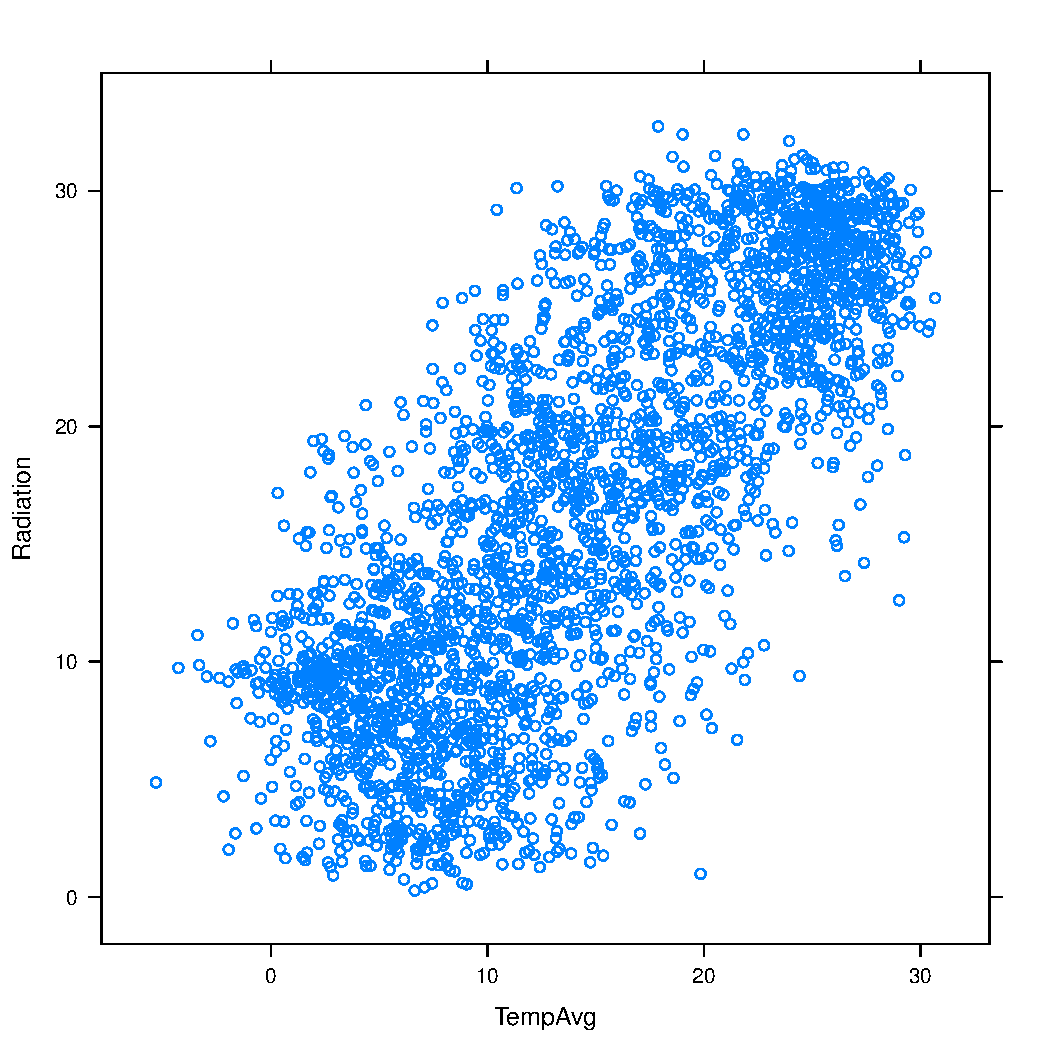
\includegraphics[width=.9\linewidth]{figs/xyplot.pdf}
\end{frame}



\begin{frame}[fragile,label=sec-6-1-4]{Añadimos regresión lineal}
 \lstset{language=R,label= ,caption= ,numbers=none}
\begin{lstlisting}
  xyplot(Radiation ~ TempAvg, data=aranjuez,
         type=c('p', 'r'), grid = TRUE,
         lwd=2, col.line='black')
\end{lstlisting}
\end{frame}

\begin{frame}[label=sec-6-1-5]{}
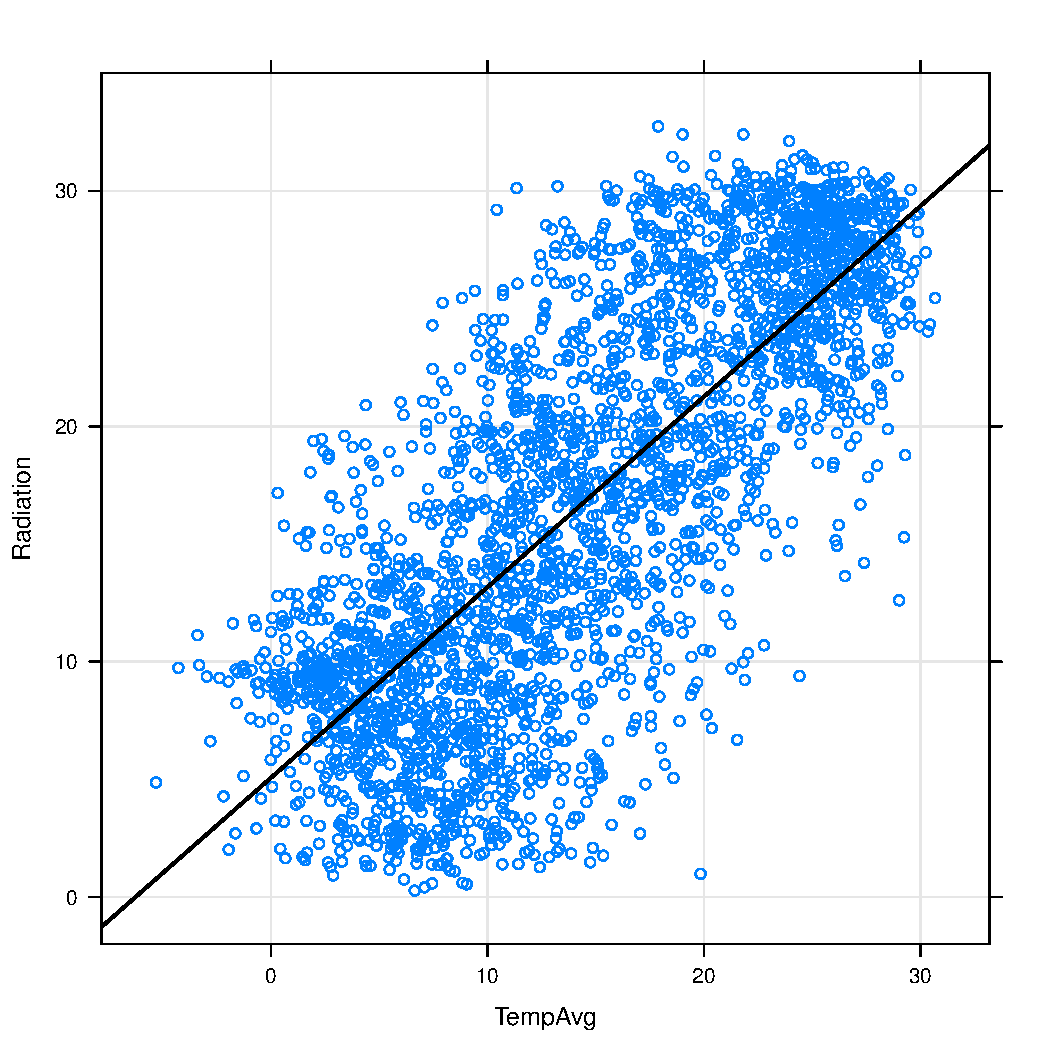
\includegraphics[width=.9\linewidth]{figs/xyplotPRG.pdf}
\end{frame}



\begin{frame}[fragile,label=sec-6-1-6]{Añadimos ajuste local}
 \lstset{language=R,label= ,caption= ,numbers=none}
\begin{lstlisting}
  xyplot(Radiation ~ TempAvg, data=aranjuez,
         type=c('p', 'smooth'), grid = TRUE,
         lwd=2, col.line='black')
\end{lstlisting}
\end{frame}

\begin{frame}[label=sec-6-1-7]{}
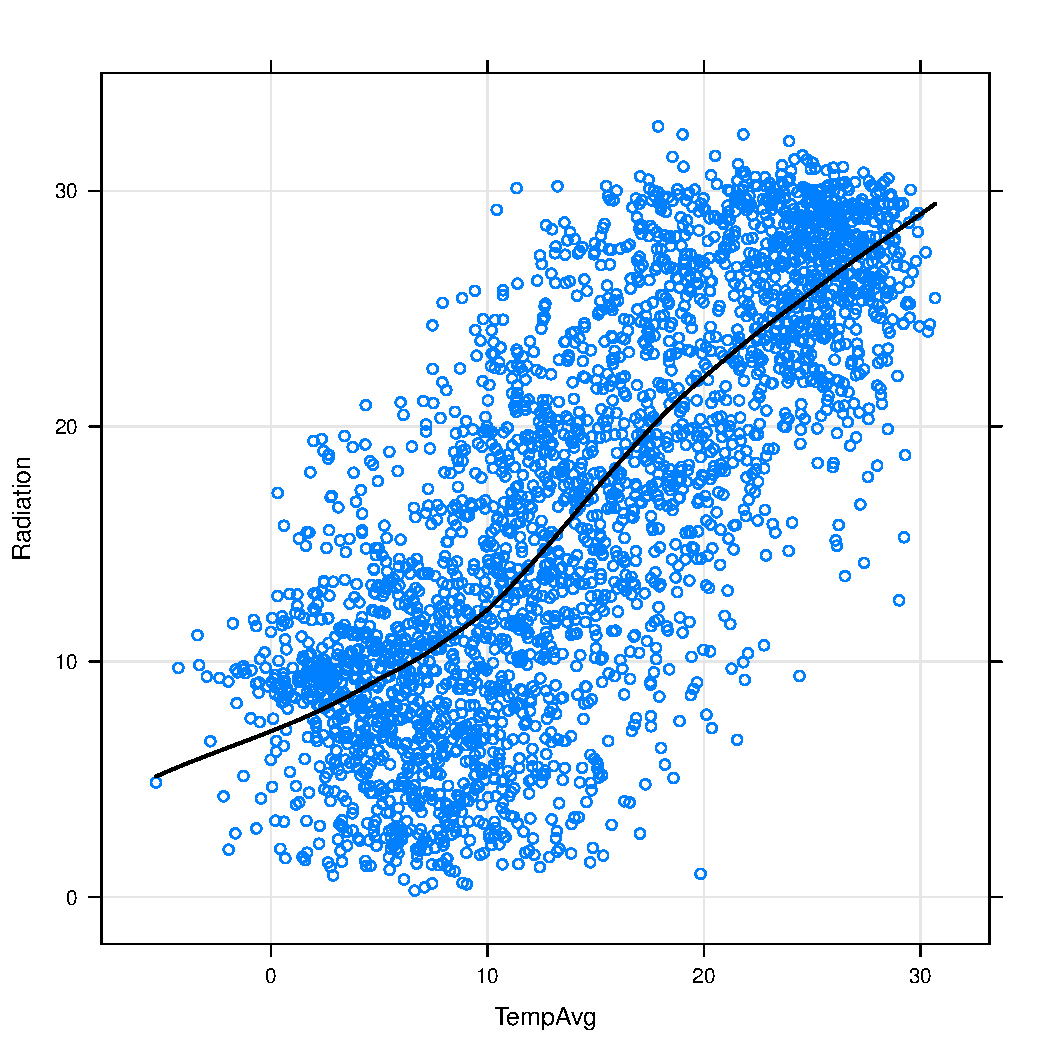
\includegraphics[width=.9\linewidth]{figs/xyplotSmooth.pdf}
\end{frame}


\begin{frame}[fragile,label=sec-6-1-8]{Paneles}
 \lstset{language=R,label= ,caption= ,numbers=none}
\begin{lstlisting}
  xyplot(Radiation ~ TempAvg|factor(year),
         data=aranjuez)
\end{lstlisting}
\end{frame}

\begin{frame}[label=sec-6-1-9]{}
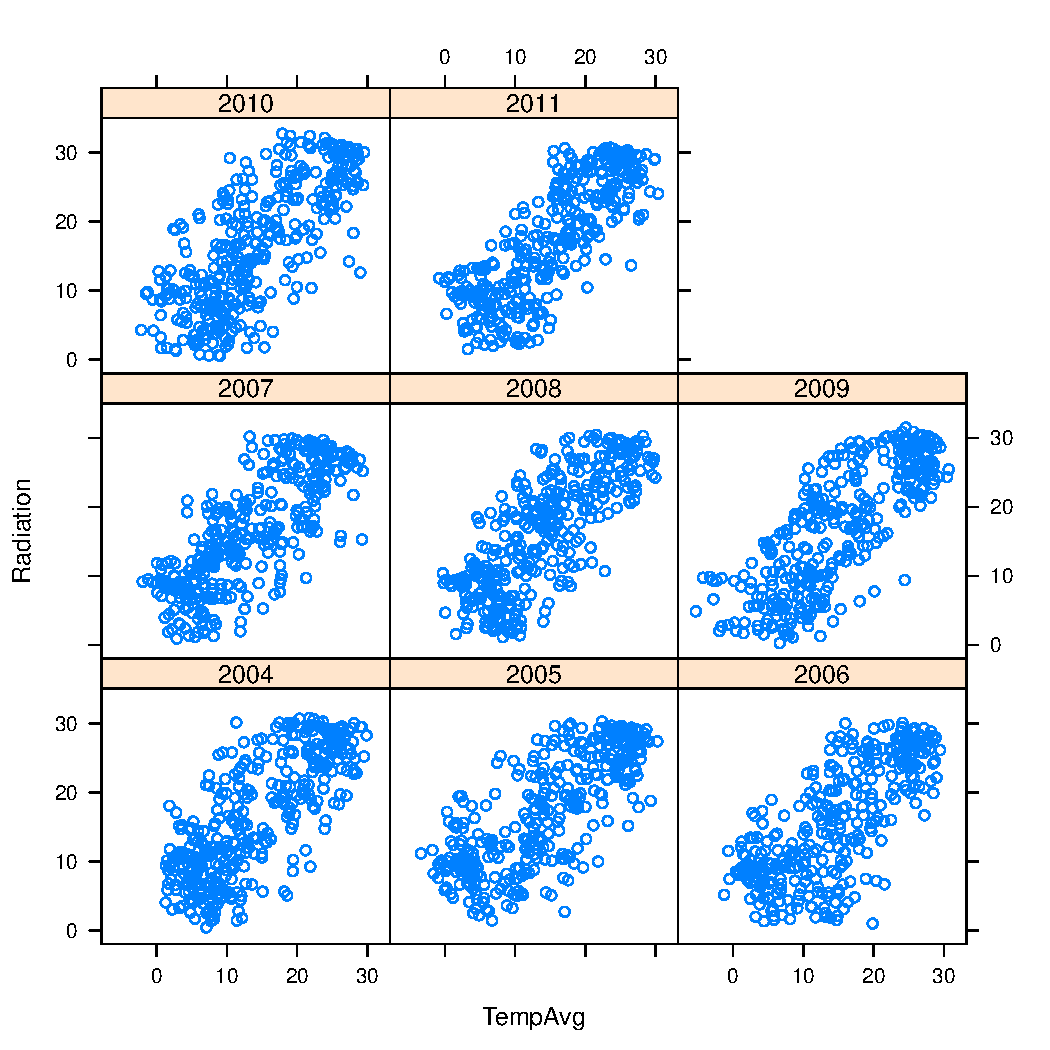
\includegraphics[width=.9\linewidth]{figs/xyplotYear.pdf}
\end{frame}

\begin{frame}[fragile,label=sec-6-1-10]{Grupos}
 \lstset{language=R,label= ,caption= ,numbers=none}
\begin{lstlisting}
  xyplot(Radiation ~ TempAvg, groups=quarter,
         data=aranjuez, auto.key=list(space='right'))
\end{lstlisting}
\end{frame}

\begin{frame}[label=sec-6-1-11]{}
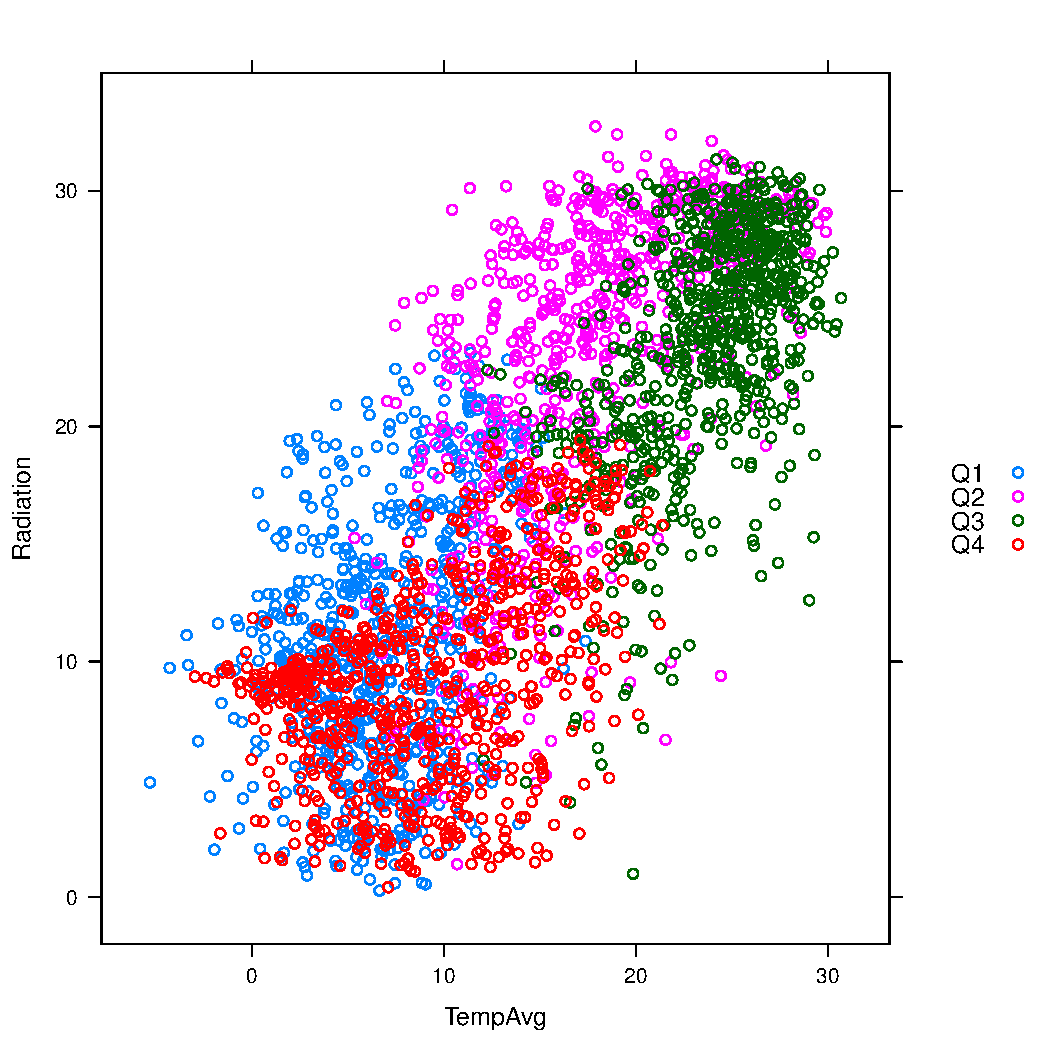
\includegraphics[width=.9\linewidth]{figs/xyplotQuarter.pdf}
\end{frame}

\begin{frame}[fragile,label=sec-6-1-12]{Colores y tamaños}
 \lstset{language=R,label= ,caption= ,numbers=none}
\begin{lstlisting}
  xyplot(Radiation ~ TempAvg,
         type=c('p', 'r'),
         cex=2, col='blue',
         alpha=.5, pch=19,
         lwd=3, col.line='black',
         data=aranjuez)
\end{lstlisting}
\end{frame}

\begin{frame}[label=sec-6-1-13]{}
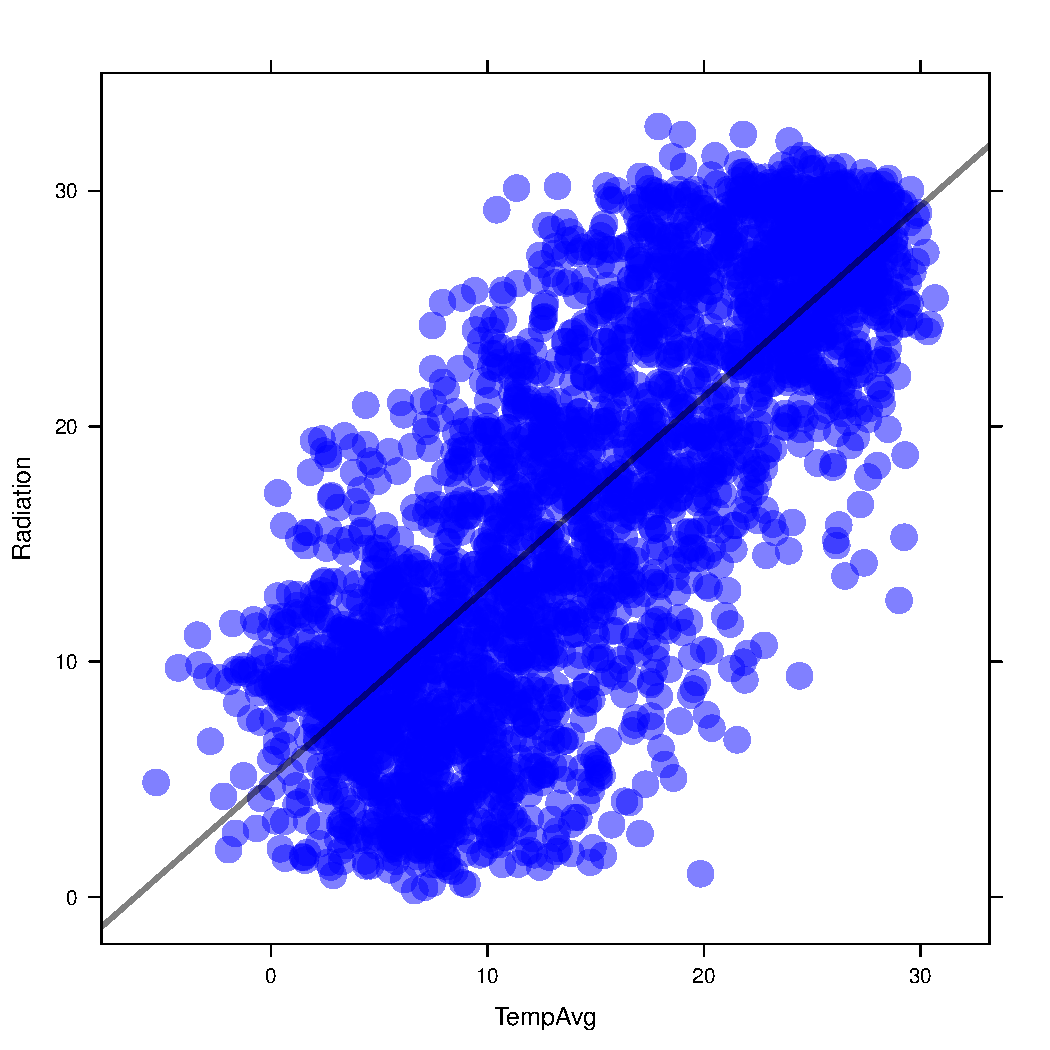
\includegraphics[width=.9\linewidth]{figs/xyplotColors.pdf}
\end{frame}

\begin{frame}[fragile,label=sec-6-1-14]{Colores con grupos: \texttt{par.settings} y \texttt{simpleTheme}}
 \begin{itemize}
\item Primero definimos el tema con \texttt{simpleTheme}
\end{itemize}
\lstset{language=R,label= ,caption= ,numbers=none}
\begin{lstlisting}
  myTheme <- simpleTheme(col=c('red', 'blue',
                          'green', 'yellow'),
                          pch=19, alpha=.6)
\end{lstlisting}
\end{frame}

\begin{frame}[fragile,label=sec-6-1-15]{Colores con grupos: \texttt{par.settings} y \texttt{simpleTheme}}
 \begin{itemize}
\item Aplicamos el resultado en \texttt{par.settings}
\end{itemize}
\lstset{language=R,label= ,caption= ,numbers=none}
\begin{lstlisting}
  xyplot(Radiation ~ TempAvg,
         groups=quarter,
         par.settings=myTheme,
         auto.key=list(space='right'),
         data=aranjuez)
\end{lstlisting}
\end{frame}

\begin{frame}[label=sec-6-1-16]{}
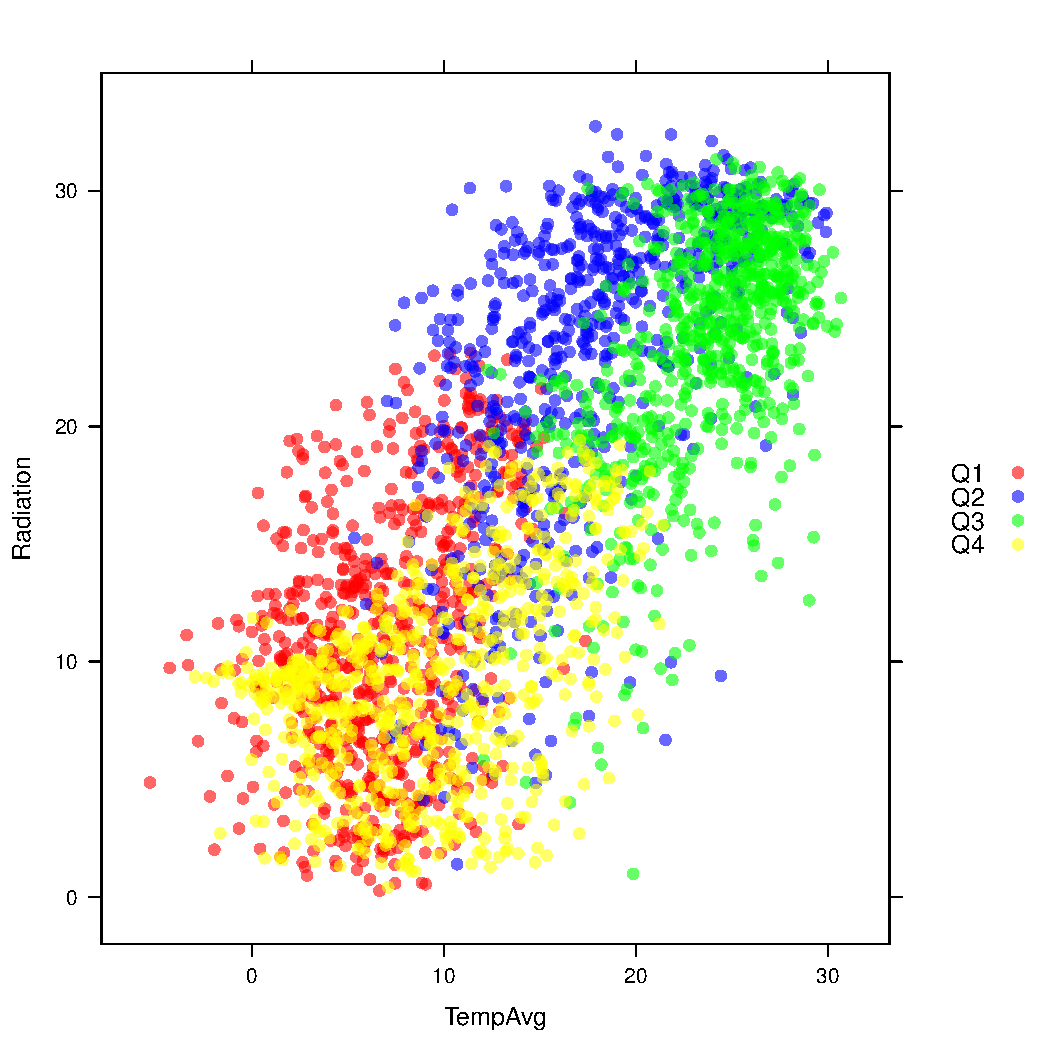
\includegraphics[width=.9\linewidth]{figs/myTheme.pdf}
\end{frame}

\begin{frame}[fragile,label=sec-6-1-17]{Colores: brewer.pal}
 \lstset{language=R,label= ,caption= ,numbers=none}
\begin{lstlisting}
library(RColorBrewer)

myPal <- brewer.pal(n = 4, 'Dark2')

myTheme <- simpleTheme(col = myPal,
                       pch=19, alpha=.6)
\end{lstlisting}

\begin{block}{ColorBrewer: \url{http://colorbrewer2.org/}}
\end{block}
\end{frame}

\begin{frame}[fragile,label=sec-6-1-18]{Asignamos paleta con \texttt{par.settings}}
 \lstset{language=R,label= ,caption= ,numbers=none}
\begin{lstlisting}
xyplot(Radiation ~ TempAvg,
       groups=quarter,
       par.settings=myTheme,
       auto.key=list(space='right'),
       data=aranjuez)
\end{lstlisting}
\end{frame}

\begin{frame}[label=sec-6-1-19]{}
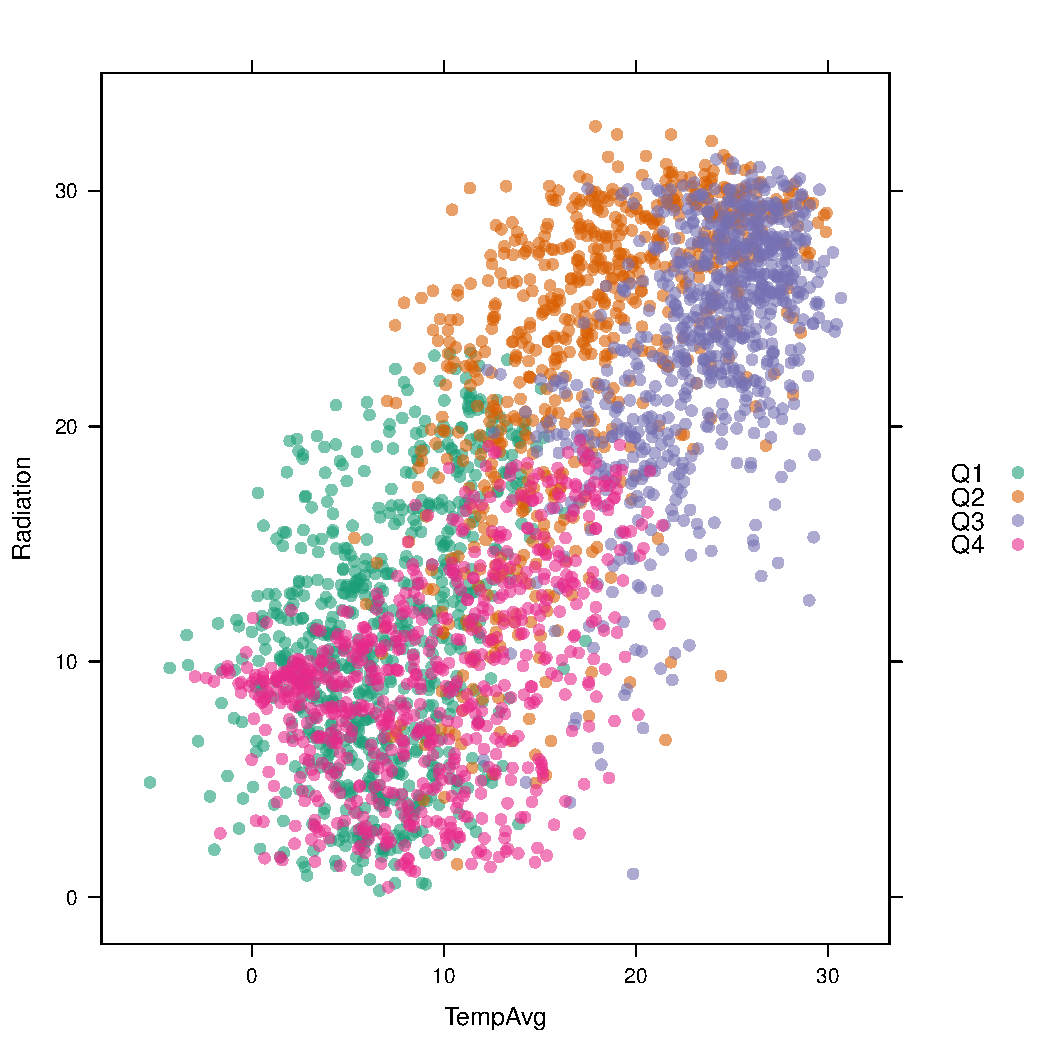
\includegraphics[width=.9\linewidth]{figs/brewer.pdf}
\end{frame}


\begin{frame}[fragile,label=sec-6-1-20]{Matriz de gráficos de dispersión}
 \lstset{language=R,label= ,caption= ,numbers=none}
\begin{lstlisting}
  splom(aranjuez[,c("TempAvg", "HumidAvg", "WindAvg",
                    "Rain", "Radiation", "ET")],
        pscale=0, alpha=0.6, cex=0.3, pch=19)
\end{lstlisting}
\end{frame}

\begin{frame}[label=sec-6-1-21]{}
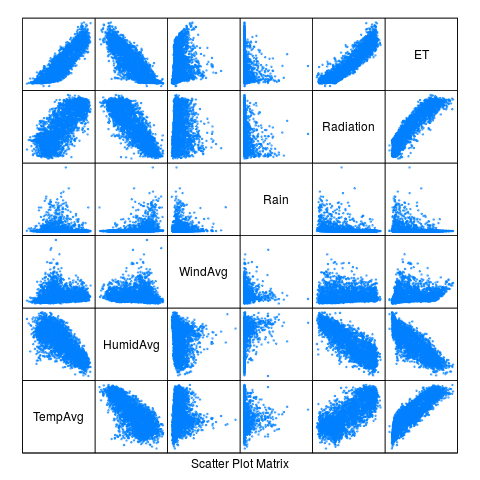
\includegraphics[width=.9\linewidth]{figs/splom.png}
\end{frame}

\begin{frame}[fragile,label=sec-6-1-22]{Matriz de gráficos de dispersión}
 \lstset{language=R,label= ,caption= ,numbers=none}
\begin{lstlisting}
  splom(aranjuez[,c("TempAvg", "HumidAvg", "WindAvg",
                    "Rain", "Radiation", "ET")],
        groups=aranjuez$quarter,
        auto.key=list(space='right'),
        pscale=0, alpha=0.6, cex=0.3, pch=19)
\end{lstlisting}
\end{frame}

\begin{frame}[label=sec-6-1-23]{}
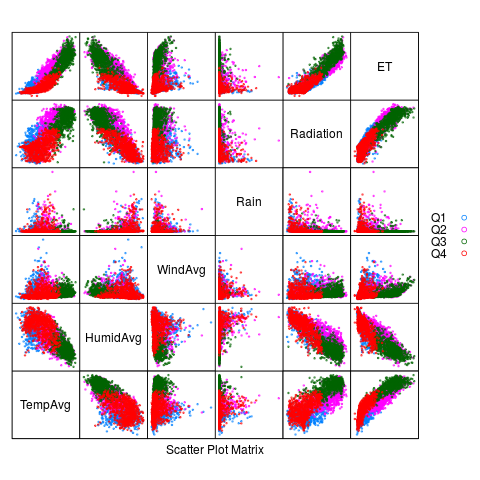
\includegraphics[width=.9\linewidth]{figs/splomGroup.png}
\end{frame}

\begin{frame}[fragile,label=sec-6-1-24]{Box-and-Whiskers}
 \lstset{language=R,label= ,caption= ,numbers=none}
\begin{lstlisting}
  bwplot(Radiation ~ month, data=aranjuez,
         horizontal=FALSE, pch='|')
\end{lstlisting}
\end{frame}

\begin{frame}[label=sec-6-1-25]{}
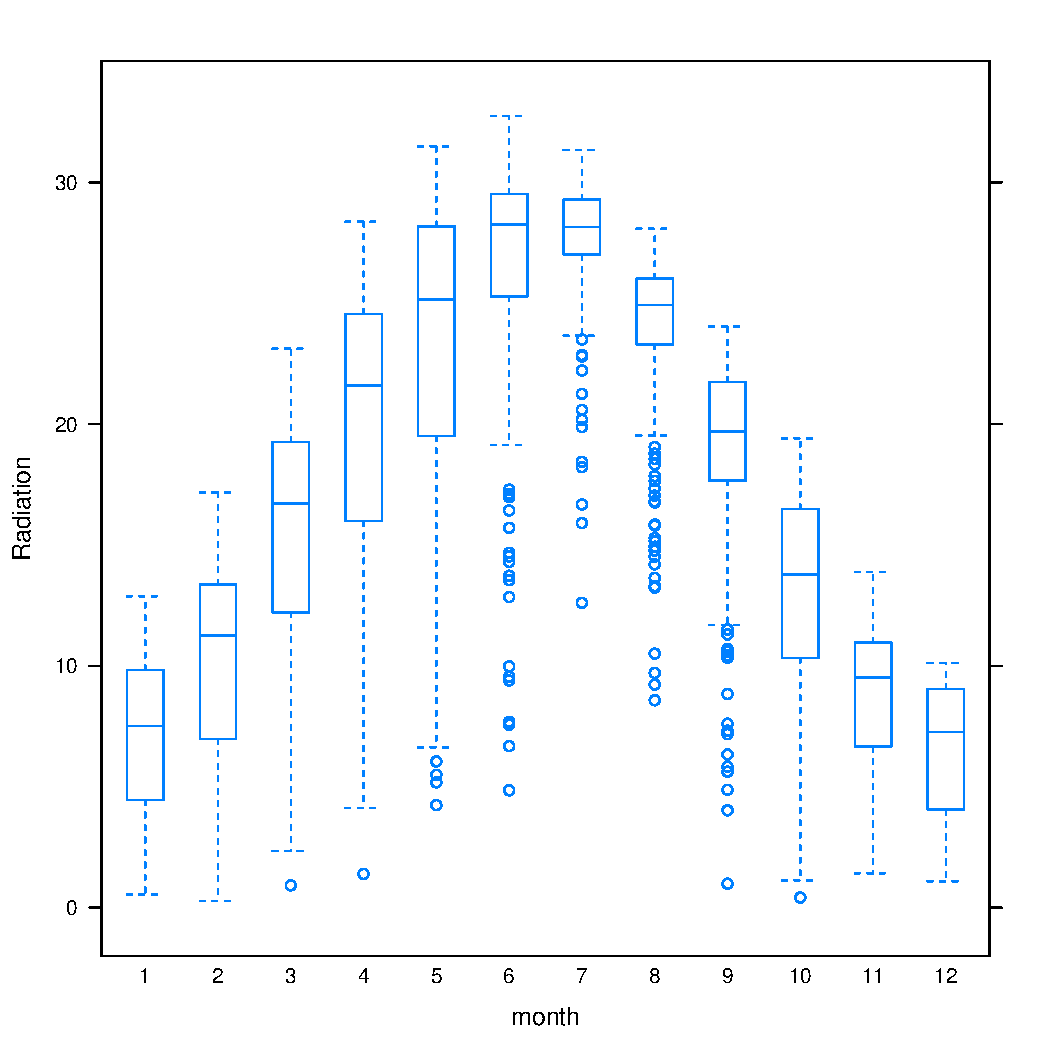
\includegraphics[width=.9\linewidth]{figs/bwplot.pdf}
\end{frame}

\begin{frame}[fragile,label=sec-6-1-26]{Histogramas}
 \lstset{language=R,label= ,caption= ,numbers=none}
\begin{lstlisting}
  histogram(~ Radiation|factor(year), data=aranjuez)
\end{lstlisting}
\end{frame}

\begin{frame}[label=sec-6-1-27]{}
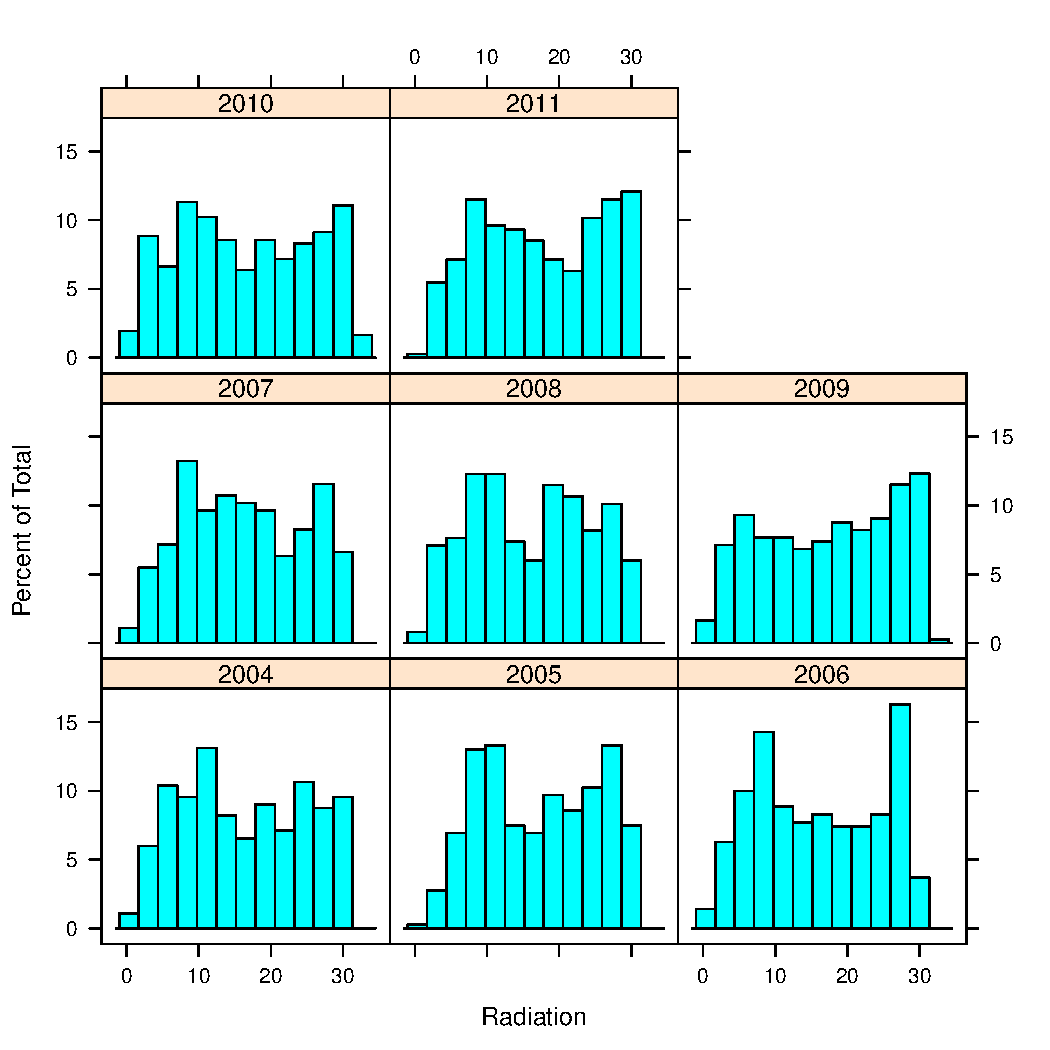
\includegraphics[width=.9\linewidth]{figs/histogram.pdf}
\end{frame}

\begin{frame}[fragile,label=sec-6-1-28]{Gráficos de densidad}
 \lstset{language=R,label= ,caption= ,numbers=none}
\begin{lstlisting}
densityplot(~ Radiation, groups=quarter,
            data=aranjuez,
            auto.key=list(space='right'))
\end{lstlisting}
\end{frame}

\begin{frame}[label=sec-6-1-29]{}
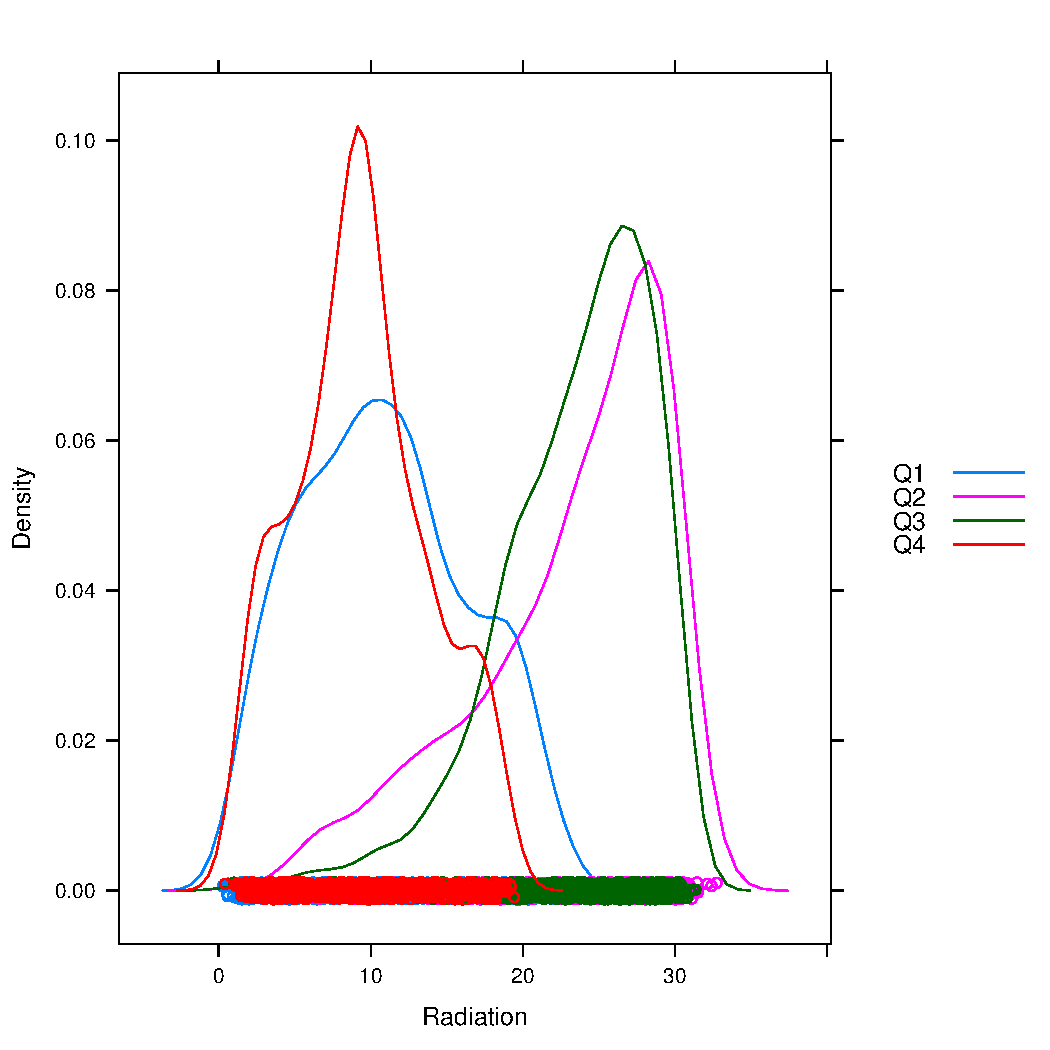
\includegraphics[width=.9\linewidth]{figs/density.pdf}
\end{frame}
% Emacs 24.4.1 (Org mode 8.2.7c)
\end{document}